\documentclass[letterpaper,12pt, spanish, oneside]{book} %%b5paper openright letterpaper
\linespread{1.5}

\let\oldfootnote\footnote
\renewcommand{\footnote}[1]{%
  \begingroup%
  \linespread{1.2}% 
  \oldfootnote{#1}%
  \endgroup%
}
\usepackage{float}  %% floating figures
\usepackage{amsfonts}
\usepackage[spanish]{babel}
\selectlanguage{spanish}

%% Setting up the header
\usepackage{fancyhdr}

\pagestyle{fancy}{
 \fancyhead[L]{\fontsize{12}{12}
 }
\usepackage{booktabs}	 		%% Tablas
\usepackage{graphicx}
\graphicspath{ {images/} }

\usepackage{lmodern} 			%% Latin modern, incluye acentos locos
\usepackage[utf8x]{inputenc}		%%Codificación utf8, requerido en la configuración
\usepackage[T1]{fontenc}			%%
%\pdfinfo{

\usepackage[nottoc]{tocbibind}

%% adjusting images
\usepackage[export]{adjustbox}

%% URL
\usepackage{hyperref}
\usepackage{xcolor}
\hypersetup{
    colorlinks,
    linkcolor={gray!50!black},
    citecolor={gray!50!black},
    urlcolor={gray!80!black}
}

\usepackage{listings}
\usepackage{color}
%\usepackage[usenames,dvipsnames]{color}
\definecolor{dkgreen}{rgb}{0,0.6,0}
\definecolor{gray}{rgb}{0.5,0.5,0.5}
\definecolor{mauve}{rgb}{0.58,0,0.82}
 
\lstset{ 
  language=R,                     % the language of the code
  basicstyle=\scriptsize\ttfamily, % the size of the fonts that are used for the code
  numbers=left,                   % where to put the line-numbers
  numberstyle=\tiny\color{blue},  % the style that is used for the line-numbers
  stepnumber=1,                   % the step between two line-numbers. If it is 1, each line
                                  % will be numbered
  numbersep=5pt,                  % how far the line-numbers are from the code
  backgroundcolor=\color{white},  % choose the background color. You must add \usepackage{color}
  showspaces=false,               % show spaces adding particular underscores
  showstringspaces=false,         % underline spaces within strings
  showtabs=false,                 % show tabs within strings adding particular underscores
  frame=single,                   % adds a frame around the code
  rulecolor=\color{black},        % if not set, the frame-color may be changed on line-breaks within not-black text (e.g. commens (green here))
  tabsize=2,                      % sets default tabsize to 2 spaces
  captionpos=b,                   % sets the caption-position to bottom
  breaklines=true,                % sets automatic line breaking
  breakatwhitespace=false,        % sets if automatic breaks should only happen at whitespace
  keywordstyle=\color{blue},      % keyword style
  commentstyle=\color{darkgray},   % comment style
  stringstyle=\color{green}      % string literal style
} 

\begin{document}
\title{
	{\textbf{Principios y aplicaciones de inteligencia artificial}}\\	
\normalsize{\textit{Un enfoque para la economía \\  	y otras ciencias sociales en R}}
	%El debate del Cálculo Económico, aproximaciones a la planificación económica computacional.}\\
%	{\large UNIVERSIDAD NACIONAL AUTÓNOMA DE MÉXICO}\\  
%	{\includegraphics[width=0.25\textwidth]{university.jpg}}
}
\author{\textit{Alfredo Olguín}}
\date{}

\maketitle

%%\chapter*{Resumen}

%%\chapter*{Dedicatoria}
%%\include{chapters/dedicatoria}

%%\chapter*{Declaración}

\textit{Para todo aquel \\
que la curiosidad insatisfecha \\ 
le corroe de incertidumbre 
y escepticismo. \\
}

\setcounter{tocdepth}{3} %% Insertar tabla de contenidos
\tableofcontents
%%\renewcommand*\listfigurename{Índice de gráficas}
%%economics.leanpub@gmail.com\listoffigures


%\chapter*{Agradecimientos}

\chapter{Introducción}
\begin{flushright}
\textit{“It is not quite a new industrial revolution, but is something nearly that scale. Our relationships with computers has changed. We used to program them, now we can teach them”}

Hinton (2017)
\end{flushright}

Posiblemente, gran parte de nosotros hemos escuchado que algoritmos “inteligentes” realizan operaciones en mercados bursátiles con rendimientos eficientes. También es muy probable deducir que vehículos de conducción autónoma tienen sistemas de inteligencia artificial que les permiten conducir de forma segura\footnote{Por ejemplo, los avances en conducción autónoma o asistida de Uber Technologies. \url{https://www.uber.com/cities/pittsburgh/self-driving-ubers/}}. Inclusive, algunos habrán identificado que un teléfono móvil al escuchar comandos de voz hace un reconocimiento de inteligencia artificial. Seguramente algunos de nosotros también hemos obtenido alguna noción de inteligencia artificial por medio de algún tipo de contenido literario o cinematográfico. Isaac Asimov, famoso escritor de ciencia ficción, solía incluir en sus novelas la posibilidad de un sistema de inteligencia artificial funcionando en convivencia regular con humanos e inclusive sugería que los robots podrían desarrollar estados de conciencia similar al humano. Sorprendentemente, hoy en día estos planteamientos resultan asequibles para algunos científicos y con miras a ser parte de nuestra vida cotidiana en un futuro no muy lejano según sus proyectos. Algunos de estos planteamientos explican la factibilidad de transferir la conciencia humana a un organismo robótico para mediados de este siglo. 

Dimitry Iskoev, un renombrado millonario interesado en impulsar desarrollos de inteligencia artificial tiene como objetivo financiar y desarrollar un proyecto de ambiciones cósmicas. El proyecto Avatar propone que para el año 2045 la tecnología será capaz de transferir la conciencia humana a una computadora y así, lograr longevidad perpetua de la especie humana. Aunque suene disparatado tener en unos años este tipo de tecnología, algunos avances ya son tangibles. En el 2015 se presentó la primera fase del proyecto Avatar. Aparentemente, los científicos e ingenieros encargados del proyecto logran controlar un robot antropomórfico a través de una interfaz computacional controlada con el cerebro humano, es decir, controlar a voluntad el movimiento de un androide con sólo pensarlo. Los avances del proyecto resultan tan fascinantes que algunos científicos creen que sienta las bases que subyacen la inmortalidad de la conciencia humana.

Cada día, los avances en tecnología relacionada a inteligencia artificial son impresionantes. Sin embargo, el orígen se remonta al pasado; más allá de la existencia de las computadoras como se conocen hoy en día, inclusive, este origen puede ser rastreado siglos atrás. Gran parte de las bases de inteligencia artificial que se desarrolla hoy en día, siquiera pertenecen a este o el anterior milenio. Pensadores griegos clásicos, hace más de dos mil años ya sentaban las bases de la inteligencia artificial y su discusión moderna.

Pero, ¿Cómo es posible que los orígenes de algo tecnológicamente tan especializado tengan un origen tan remoto en el tiempo?. Algunos autores aseguran que los fundamentos metodológicos de la inteligencia artificial están basados en teorías del conocimiento desde hace cientos de años, y que  algunos de los preceptos tienen orígenes desde los pensadores clásicos griegos, esto hace más de un par de milenios. 

Para entender los principios básicos de inteligencia artificial (o cualquiera de sus vertientes), es necesario conocer la forma en que los humanos adquirimos conocimiento y las razones por las cuales este conocimiento es importante. Es fundamental, pensar en términos de adquisición de conocimiento al momento de tratar de enseñar a pensar o emular la forma en que razonan los seres humanos. La ciencia que estudia la forma en que pensamos es conocida como epistemología.

El estudio del conocimiento ha sido tema central en la filosofía por siglos y dio origen a la epistemología. El término epistemología tiene origen griego y se compone de episteme (semilla) y logos (estudio). Una variedad inmensa de autores y corrientes del pensamiento componen esta diversa parte de la filosofía, en este libro sólo se menciona una minúscula pero fundamental parte de la epistemología que da orígen a los principios de inteligencia artificial. Entender la forma en que se origina el conocimiento desde la epistemología permite comprender la forma en que se presentan algunos de los paradigmas de inteligencia artificial y el porqué algunos autores consideran que tal “inteligencia” artificial no existe.

Un concepto básico que tiene siglos de discusión es sobre el origen del conocimiento. Algunos filósofos establecen que a través de los sentidos (vista, olfato, tacto etc) se obtiene información sobre lo que nos rodea. Adicionalmente a los sentidos, también plantean que de forma mental-interna los humanos obtenemos conocimiento y esto justifica la existencia de la imaginación y los sueños, por ejemplo. Flasiński (2016) establece que los primeros filósofos en distinguir entre percepción sensorial y percepción mental datan desde el siglo V (a.e.c.) con los aportes de Parménides de Elea y Platón. Más adelante, la discusión se desarrolla por parte de Aristóteles en el siglo IV (a.e.c) al contraponer los argumentos de Platón y Tomás de Aquino al desarrollar la filosofía aristotélica poco más de mil años adelante en el siglo XIII (e.c) define inteligencia como “el acto mismo del intelecto, que es el conocimiento”. Además, Tomás de Aquino ofrece distinciones entre las formas de percepción del exterior y aquellas del interior. 

René Descartes, famoso filósofo y matemático francés del siglo XVII hace una distinción sobre las operaciones meramente mecánicas y aquellas que requieren un nivel de conocimiento. 

Descartes (2002) argumenta que aquello correspondiente al pensamiento es ajeno al resto de la naturaleza o substancias corpóreas. Simplificando, res cogitans corresponde a la la sustancia que proviene del pensamiento y res extensa al resto de la naturaleza.  La influencia esencial de Descartes radica en establecer un método de adquisición del conocimiento por medio del método de razonamiento deductivo. Algunos principios de las contribuciones de Descartes aún existen como premisas metodológicas en distintos planteamientos del razonamiento que ejercen ciertos desarrollos en discusiones centrales en inteligencia artificial hoy en día. 

Tratar de identificar el origen y desarrollo histórico de los principios filosóficos de la inteligencia artificial resulta demasiado extenso y fuera de las ambiciones prácticas de este texto. Sin embargo, es importante destacar que otros filósofos cuyos planteamientos son reconocidos como relevantes para los investigadores de inteligencia artificial se encuentran a lo largo de la historia. Algunos casos destacados son Kant (1724-1804), J. Stuart Mill (1806-1873), Husserl (1859-1938) y Kurt Gödel (1906-1978) por ejemplo\footnote{Una versión detallada de los aportes filosóficos se puede encontrar en Flasiński (2016)\textit{ Theories of Intelligence in Philosophy and Psychology} y una perspectiva histórica O’Regan(2016, 2012) \textit{Introduction to the History of Computing, A brief history of Computing.}}. Sucesivamente, propuestas, planteamientos y  teorías fueron desarrolladas en el tiempo pero fue hasta mediados del 1950 que se reconoce el nacimiento del término inteligencia artificial en la famosa conferencia de Dartmouth de 1956, en Hanover Estados Unidos. De esta manera dando origen y continuidad a uno de los temas más discutidos en varias ramas de las ciencias.

A pesar de ser un tema auge desde mediados del siglo XX en otras disciplinas como ciencias computacionales, psicología, lingüística, neurociencias, medicina, física, filosofía y biología. La ciencia económica (así como otras ciencias sociales) ha tenido poco desarrollo interno sobre temas relacionados a aprendizaje automatizado. Más relevante aún, cuando uno de los creadores del primer programa de inteligencia artificial Logic Theorist, el economista Herbert Simon (1956) recibió el premio Nobel en economía de 1978.

En general, se observa poco desarrollo interdisciplinario entre la ciencia económica y los planteamientos de inteligencia artificial. Usualmente, la visión dominante que conjunta ambas disciplinas se conoce como computational economics, una rama de la economía que surge a finales del siglo XX. No obstante, gran parte de los avances en computational economics no muestran una tendencia a ser textos introductorios o de acceso común. En cambio la mayoría de los investigadores se enfocan en publicar artículos state-of-the-art o  al menos muy específicos sobre el tema. Si bien, los textos de vanguardia son sumamente importantes para el desarrollo científico, limitan el acceso a entusiastas aún no especialistas en el tema. El objetivo de este texto es permitir a estos entusiastas adquirir conocimientos teóricos y prácticos a un nivel introductorio con el fin de sembrar una semilla de curiosidad que permitirá al lector digerir textos más avanzados, así como parte de las propuestas de la economía computacional.

Una parte importante de las propuestas de economía e inteligencia artificial son el caso de las finanzas para análisis de mercados. Se puede considerar como la rama  más desarrollada de ambas disciplinas, sin embargo se reconoce como poco difundido y con un sesgo muy grande de material accesible.

Arthur Samuel (1901-1990), uno de los pioneros y colaborador del premio Nobel en economía Herbert Simon, acuñó un término sumamente relevante para estos temas. Conocido como  Machine learning o aprendizaje automatizado es una rama de las ciencias computacionales que estudia patrones en información y ofrece un método de inteligencia artificial, quizás hoy en día más popular y relevante de lo que su creador pudo imaginar.

En la actualidad, la mayoría de los libros sobre aprendizaje automatizado se enfocan en desarrollar conceptos en notación estadística y matemática. A diferencia de gran parte de los textos, este libro utiliza conceptos matemáticos básicos y un lenguaje de programación orientado al análisis económico. Así, como economista, los conceptos matemático-estadísticos resultan asequibles para analizar, y resolver problemas económicos.

A pesar de que haber una difusión amplia, las aplicaciones de estas técnicas computacionales son poco discutidas en planes de estudio básicos para economistas. Desde la perspectiva de un economista aún no experto en temas de programación o con debilidades en conceptos avanzados de modelización estadística, en este libro se podrán encontrar aplicaciones básicas que ayudan a reforzar ideas más complejas que se pueden consultar en literatura especializada en temas de aprendizaje automatizado.

Adicionalmente, se ofrece toda la documentación necesaria para empezar a crear ejemplos con información real a lo largo de cada capítulo para distintos casos de uso. A lo largo del libro, se observa una introducción paulatina de problemas simples a retos del mundo real. 

La clase de proyectos e investigaciones que un economista puede desarrollar son variados, desde análisis crecimiento macroeconómico, comercio internacional, mercados financieros etc. Este libro desarrolla un poco de cada tema con el objetivo de conocer aplicaciones en varias áreas. Por ejemplo, el capítulo X será de especial interés para aquellos cuyos temas se enfocan a las cuestiones de comercio internacional. Por ejemplo, en el capítulo tercero se ofrecen todos los pasos necesarios para predecir comportamiento de mercados mediante un sencillo modelo redes neuronales artificiales.

Una versión simplificada de análisis de minería de textos permite crear una herramienta similar a lo que usa Bloomberg en sus paneles de análisis sociales desde 2013. A través de procesamiento del lenguaje natural, se pueden analizar tendencias sobre una emisora específica. Para el capítulo Y se analizan tendencias de mensajes de \textit{twitter} en tiempo real.


\chapter{Requerimientos y sugerencias}

La estructura del libro está pensada para llevar a la práctica la mayoría de los conceptos que se presentan a lo largo del texto. El objetivo es que sea una herramienta con preponderancia práctica y fundamento teórico. Con el objeto de realizar ejercicios prácticos, se utilizará un lenguaje estadístico-computacional muy popular llamado R y conceptos básicos de econometría convencional. Para ambos casos, hay una gran cantidad de textos disponibles para comenzar y profundizar. 

Puesto que este no es un texto sobre programación en R,  los textos que recomiendo para introducción al lenguaje R son las notas de documentación oficial \textit{An Introduction to R} de Venables y Smith (2016) o la versión enfocada a la popular rama interdisciplinaria Ciencia de Datos de Peng (2016) \textit{R programming for Data Science}. Ambos textos de acceso libre y con actualizaciones periódicas según los autores. 

No obstante, aquí se presenta una introducción general con ayuda de la librería swirl.  El paquete ofrece una forma interactiva para comenzar a utilizar la herramienta desde cero y bien, podría servir como mínimo indispensable para familiarizarse con el ambiente de trabajo en R. Una vez concluída la instalación del lenguaje, se puede comenzar a explorar por este medio como se explicará a continuación. 

\subsection{Instalación del lenguaje}

Aunque no es requisito indispensable tener un amplio manejo de lenguajes de programación para conocer los principios de inteligencia artificial aplicados, se recomienda seguir los ejercicios para tener un fundamento práctico. En este apartado explicaremos la instalación de ambientes (instalación de los programas) que nos permitirán dar seguimiento al contenido del libro.

El lenguaje está disponible para las plataformas más comunes Windows, Linux y Mac en el repositorio oficial https://cran.r-project.org. Como se ejemplifica en la figura siguiente, de lado derecho seleccionamos la distribución que nuestro ordenador opera y seguimos las instrucciones de instalación. Para el caso más común de  Windows, se detallan a continuación.

\begin{figure}[H]
\centering
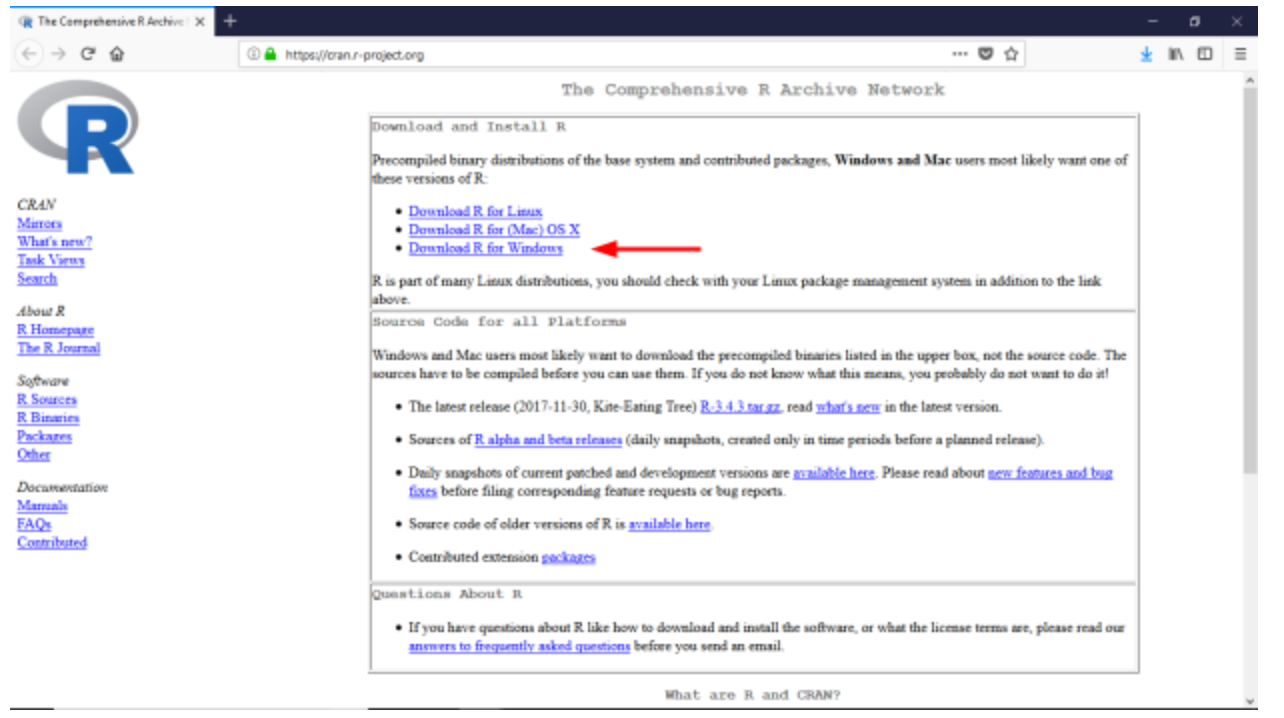
\includegraphics[width=0.7\textwidth]{t1.png}
\caption{\label{fig:frog2}\textit{Se da click en la instalación del sistema operativo que corresponda. En este caso Windows}.}
\end{figure}

De lado derecho seleccionamos la distribución que nuestro ordenador opera y seguimos las instrucciones de instalación. Para el caso más común de  Windows, se detallan a continuación.

\begin{figure}[H]
\centering
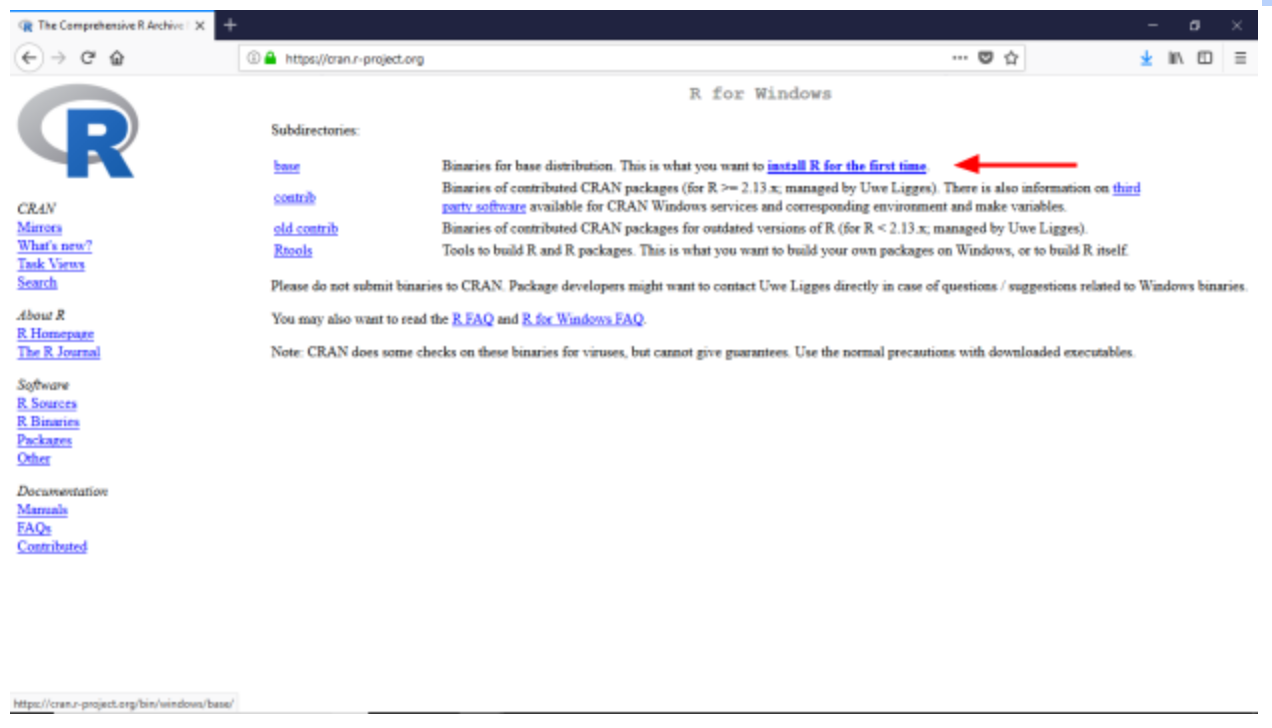
\includegraphics[width=0.7\textwidth]{t2.png}
\caption{\label{fig:frog2}\textit{Dando click en la instalación comenzará la descarga del programa. Para completar la instalación dar en siguiente a la configuración sugerida}.}
\end{figure}

Una vez ejecutado el instalador, seleccionado el lenguaje, todos los componentes  una ventana nos confirmará que hemos instalado adecuadamente el lenguaje. Posteriormente, instalaremos una interfaz que nos ofrecerá una versión gráfica amigable para el usuario. Aunque se puede trabajar únicamente con el lenguaje R, la interfaz de usuario permitirá manejar R de forma más natural, se incluyen funcionalidades útiles al momento de ejecutar, probar y guardar comandos.

\subsection{Instalación de interfaz de usuario Rstudio}

Con creces el ambiente gráfico más popular de R es \textit{Rstudio}. Esta herramienta ofrece una variedad de soluciones más avanzadas que servirá para aquel entusiasta que quiera profundizar en visualizaciones dinámicas (\textit{Rstudio Shiny}) o la versión que se ejecuta para un servidor (\textit{Rstudio Server}). Sin embargo, en este caso solamente ocuparemos la versión de escritorio (\textit{Desktop}) a través del sitio oficial https://www.rstudio.com/products/rstudio/download/ y eligiendo la distribución correspondiente a nuestro sistema operativo. En este caso, Windows. 

\begin{figure}[H]
\centering

\includegraphics[width=0.7\textwidth]{t3.png}
\caption{\label{fig:frog2}\textit{Se selecciona la versión para Windows Vista/7/8/10 para descargar. Al terminar, se ejecuta el archivo y se siguen las opciones predeterminadas }.}
\end{figure}

Una vez terminada la descarga, seguiremos los pasos sugeridos de instalación. El asistente de instalación confirmará que se haya logrado configurar el programa y todo estará listo para trabajar.

Al abrir Rstudio se mostrará un ambiente similar al siguiente. En la sección 1 se tiene el espacio dedicado a la construcción de un script y notas. En la sección 2 se tiene la consola, el espacio donde se ejecutan los comandos. En la sección 3 está el ambiente donde se visualizan los datos y funciones que definimos. Por último, en la sección 4 se describen las carpetas y archivos en nuestro ambiente, las gráficas que se generan, los paquetes instalados y una ventana de ayuda de documentación sobre los paquetes instalados.

\begin{figure}[H]
\centering
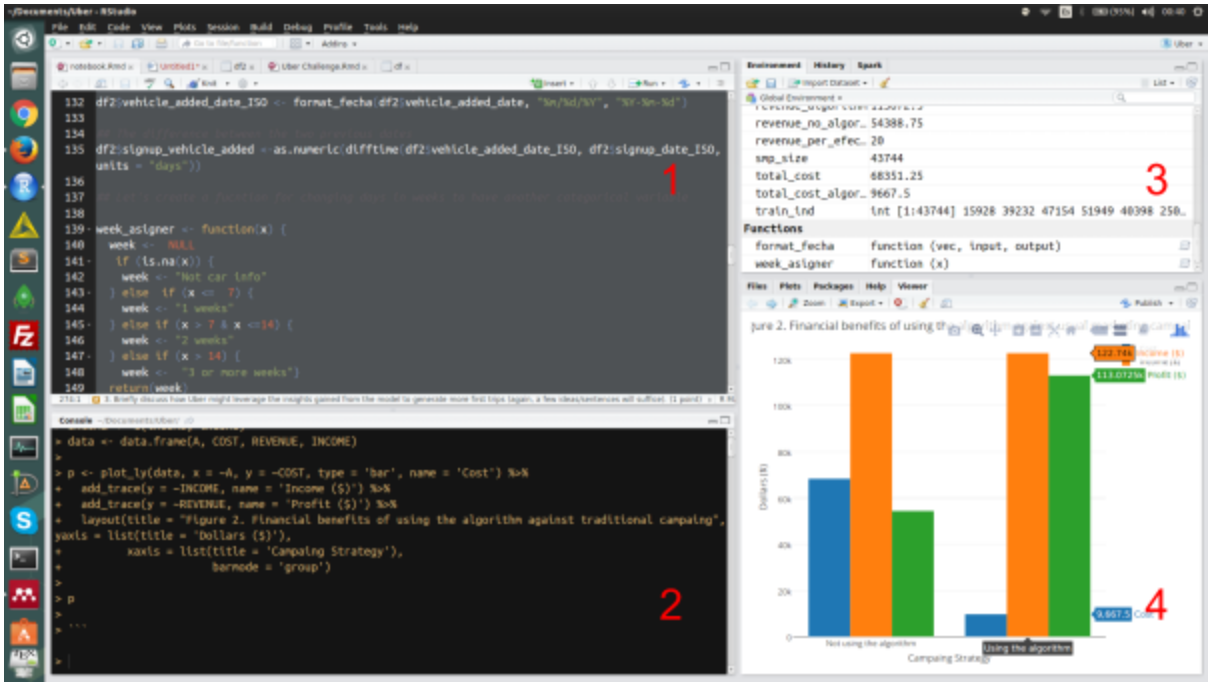
\includegraphics[width=0.7\textwidth]{t4.png}
\caption{\label{fig:frog2}\textit{Se selecciona la versión para Windows Vista/7/8/10 para descargar. Al terminar, se ejecuta el archivo y se siguen las opciones predeterminadas }.}
\end{figure}

\subsection{Nociones Básicas, aprendiendo R con swirl}
Al finalizar la instalación de los ambientes, se puede proceder a explorar el lenguaje. Una forma fácil, interactiva y entretenida de hacerlo es por medio del paquete \textit{swirl}. 

\begin{lstlisting}
## Instalacion de swirl
install.packages("swirl")

## Cargando libreria
library("swirl")

## Iniciando el tutorial
swirl()
\end{lstlisting}

Una vez ejecutados los comandos swirl explicará los principios básicos de R y de forma interactiva el usuario debe responder las preguntas que el sistema arroja . En la lección 1 se revisan los conceptos básicos del lenguaje. En la lección dos se ven modelos simples de regresión lineal. En la lección tres estadística inferencial básica y en la lección cuatro análisis exploratorio.

Aunque terminar todas las lecciones sería beneficioso para cualquiera, para este libro los conceptos fundamentales de swirl en la lección 1 y 2 son suficientes para comenzar en buena forma. 

¡Felicidades! si has llegado hasta aquí puedes considerar que ya conoces los ambientes y estás listo para embarcarte en ambiciosos análisis de inteligencia artificial en R. A lo largo del desarrollo del texto, se utilizarán varios de los temas comunes, no obstante, con algo de experiencia el usuario de R notará que existen diferentes formas de llegar a los mismos resultados y la forma de definir los comandos no son únicas ni universales.

\section{Material adicional y cómo trabajar con el código}

A lo largo del texto, se mostrarán seccione de código. Todo el material descrito puede ser descargado de manera gratuita del sitio web \url{https://github.com/alfredo203/economia_inteligencia_artificial}. Si se es un usuario de Git, el mismo sitio web da la posibilidad de descargar el repositorio completo. El repositorio está organizado por capítulos y cada capítulo está dividido por secciones de código por subcapítulo. 

\section{Contacto}

Gran parte de este libro es un proyecto que se encuentra en progreso, en proceso de cambios y mejoras continuas. Agradeceremos cualquier duda o comentario respecto al libro que nos ayude a mejorar el contenido en siguiente correo electrónico \href{mailto:me@somewhere.com}{economics.leanpub@gmail.com} .

En caso de encontrar una falla en el código, puedes levantar un ticket en el repositorio oficial del texto en Github \url{https://github.com/alfredo203/economia_inteligencia_artificial/issues.}

\chapter{Principios básicos de aprendizaje automatizado}
\begin{flushright}
\textit{“The first obvious fact about human learning is that it’s horribly slow. It takes decades for human beings to learn anything. It took all of us six years just to get up to starting speed for school, and then twenty more years to become cognitive scientists or computer scientists. That’s the minimum, some of us took even longer than that. So we are terribly slow learners...”}

Herbert Simon (1983)
\end{flushright}

En la actualidad, el aprendizaje automatizado es una pieza fundamental para distintas áreas del conocimiento e industrias a través del mundo. Hoy en día, una gran parte de nuestra vida diaria está regida por algoritmos de inteligencia artificial que realizan cálculos específicos para obtener una recomendación de producto en una tienda en línea, conocer una película que nos agradará o elegir la ruta más adecuada en un sistema de GPS. Por ejemplo, al mostrar interés en un producto la publicidad de Amazon el sitio web constantemente enviará publicidad y recomendaciones relacionadas a ese artículo específico. Al terminar de ver una película, el sistema de recomendación de Netflix nos sugiere un título nuevo en función de un análisis del patrón de gustos de películas vistas con anterioridad. Al seleccionar una ruta preferida, el sistema GPS recomendará la elección previa y posiblemente recomendará a otros conductores la ruta sugerida si es más eficiente. Para los teléfonos celulares y buscadores web, un algoritmo enfocado en semántica de texto completa nuestras búsquedas, nos sugiere nuevas palabras en función de nuestro uso cotidiano del lenguaje y la forma en que la sociedad realiza las búsquedas.    

Así como los ejemplos mencionados un sinfín de aplicaciones nos rodean diariamente, el mundo digital basa gran parte de su desempeño en la capacidad de adaptar algoritmos específicos a necesidades específicas. Algunos de los ejemplos que subyacen a estas necesidades se engloban en las siguientes acciones.

\begin{description}
\item [$\bullet$ Segmentar:] Agrupar o dividir en secciones homogéneas.
\item [$\bullet$ Identificar:] Determinación características o factores.
\item [$\bullet$ Predecir:] Pronosticar, realizar una conjetura con antelación.
\end{description}

En general, la mayoría de los casos de uso de inteligencia artificial se enfocan en las aplicacione anteriores. Un centro de estudios médicos estará muy interesado en \textbf{identificar} los factores que incrementan el riesgo de padecer infarto cardiaco (Easton, 2014). Un analista de bolsa estará interesado en \textbf{predecir} los precios de las emisoras más rentables en el mercado (Dunis et al, 2016). Tomadores de decisiones de política monetaria podrían \textbf{segmentar} los sectores más propensos a sufrir un alza de inflación dado un shock de precios, entre un sin fin de casos de uso.

Mediante herramientas de aprendizaje automático es posible enseñar a una computadora a realizar tareas sencillas de segmentación, identificación y predicción. Así, la segmentación de una campaña para clientes específicos dados ciertas necesidades, gustos y preferencias es posible utilizando algunos principios de inteligencia artificial.\footnote{Dentro de la economía este tipo de análisis todavía no está generalizado y los casos son bastante exiguos. Un caso de segmentación de campaña, procesamiento de lenguaje natural y teoría económica se muestra en los trabajos previos Olguín (2016).}

Ejemplificando, supongamos que tenemos una que no tiene conocimiento de los peligros al recorrer una acera cualquiera. Lamentablemente el individuo no conoce nada sobre el mundo real y su única función actual es caminar en línea recta. Para simplificar, supongamos también, que esta acera es infinita y esta persona caminará un tiempo indefinido por ella. Para fortuna de este individuo la acera es perfecta y no hay algún tipo de impedimento que le cause dificultades, pero lamentablemente, un día en una sección de la acera aparece un agujero. El individuo al no conocer el riesgo, decide continuar con sus funciones de caminar en línea recta y cae en el agujero. Al caer en este hipotético agujero, el sujeto en cuestión tendrá un estímulo negativo (quizás dolor o miedo), el sujeto identificará de manera automática un agujero con estas experiencias negativas y en la mayoría de los casos evitará caer en cualquier agujero futuro. El sujeto, así como cualquier sistema artificial (ante un estímulo) \textit{aprende}.

\section{Nociones básicas de aprendizaje supervisado y no supervisado}

Para la terminología tradicional de machine learning, el aprendizaje supervisado es un concepto que se utiliza para designar un tipo de información. Se hace llamar aprendizaje supervisado a toda aquella información que está etiquetada ex ante un algoritmo o técnica estadística interfiera para predecir su comportamiento. Generalmente representado en vectores podemos tener un vector de objetos que tienen características binarias\footnote{Para un econometrista experimentado, observará que dummies variables siguen este principio. Para una introducción simple, el texto \textit{Basic Econometrics} de Gujarati (2012) ilustra claramente las variables dicotómicas y sus usos en la modelación econométrica.} (género femenino / género masculino, si / no, empleado / no empleado, pobreza / no pobreza). 

En el caso de aprendizaje supervisado, las variables que contienen información que ayuda a desarrollar un modelo estadístico con esta información \textit{ex ante}. Siendo aprendizaje no-supervisado la información no estará disponible, es decir, no se conocerá si un individuo pertenece a una categoría determinada u otra. 

Un ejemplo típico de aprendizaje no supervisado que gran parte de los científicos sociales reconocerán es el caso de medición de pobreza en función de características de la vivienda y la familia que la habita. En el caso más simple que podemos ejemplificar el siguiente caso. Analistas determinarán que bajo ciertos criterios de ingreso, acceso a educación y a servicios cierta vivienda estará en estado de pobreza o no. Los analistas encargados de determinar si pertenece a cierto grupo no conocerán ex ante si un hogar pertenece a una vivienda en situación de pobreza y se enfrentan a un problema de aprendizaje no supervisado.

Usualmente, se considera que los problemas de aprendizaje no supervisado son más complejos y avanzados de desarrollar. Aunque en casos más simples los algoritmos de aprendizaje no supervisado no son avanzados y requieren un entendimiento básico de estadística convencional.

Principalmente, este libro se enfocará en mostrar aplicaciones a aprendizaje supervisado y versiones sencillas de aprendizaje no supervisado al ser un texto introductorio. Para esta primera sección del texto se revisan los conceptos básicos de una regresión lineal desde el punto de vista práctico. Se analiza el primer caso de regresión lineal de la historia y se compara con álgebra lineal simple para conocer las similitudes. Segundo, se utiliza el modelo de regresión lineal para hacer un caso de segmentación de aprendizaje supervisado. 

\subsection{Introducción a modelización y clasificación lineal}

En general, los métodos de regresión lineal han estado en el núcleo de las herramientas de gran parte de los científicos sociales durante mucho tiempo. A pesar de ser técnicas consideradas como simples, demuestran un desempeño bastante aceptable para una gran cantidad de aplicaciones e inclusive un desempeño mucho mejor en casos donde la información es escasa o con problemas de sesgo estadístico.

Esta sección puede considerarse como los fundamentos básicos que se esconden detrás de sistemas de inteligencia artificial para una gran cantidad de casos. Para todo aquel que quiera utilizar herramientas avanzadas, es importante conocer los cimientos de conceptos básicos que se trabajarán en las secciones siguientes, algunos algoritmos de agrupamiento \textit{clustering} y técnicas de aprendizaje como redes neuronales tienen en su núcleo teórico fundamentos de regresión lineal simple.

En esta sección, revisaremos estos fundamentos básicos que componen una regresión lineal partiendo de la práctica; aplicando un modelo de regresión lineal desde el inicio. Se genera un modelo estadístico univariado y se genera una demostración empírica-gráfica de que el modelo de regresión lineal simple univariado representa la misma función estimada que una ecuación de la recta convencional (y = mx + b).

\subsection{Análisis de regresión lineal}

Sin duda el análisis de regresión lineal es la técnica más conocida en el campo de estadística y algunas otras disciplinas. En su versión más simple, esta consiste en observar la relación entre dos variables o vectores. Para todo modelo de regresión lineal existe una variable dependiente que llamaremos $Y$ y consiste en la variable que queremos predecir. Por otro lado las variables independientes las llamaremos $X_i$ y consisten en las variables que se utilizan para explicar $Y$. Matemáticamente, la ecuación que explica estas relaciones es la siguiente.

$$\hat{Y} = b_0 \ + b_1 X_1 \ + b_1 X_2 \ ... b_i X_i$$

Dónde $\hat{Y}$ es la estimación de Y que se efectúa en el modelo, $b_1$ … $b_i$ son los estimadores y $X_i$ las variables que se utilizan para explicar $Y$. $B_0$ es llamado intercepto.

Aunque a simple vista el modelo de regresión lineal pueda parecer un poco complicado de asimilar a primera vista, conocer un poco de su historia sirve para comprender cómo surgió la idea y entender el caso concreto donde se utilizó por primera vez.

\subsubsection{Regresión a la \textit{medocridad}, origen de la regresión lineal}

En realidad la regresión lineal, es un método de estimación más viejo de lo que aparenta ya que tiene su origen en el siglo XIX. Francis Galton, primo del naturalista Charles Darwin, es conocido por sus aportes como sociólogo,  estadístico, biólogo y reconocido científico en varias ramas. A finales del siglo XIX, Galton utiliza un método de regresión lineal para explicar una hipótesis simple que formó a partir de la observación. Tras estudiar una clase específico de planta llamado Lathyrus odoratus, se percató que las semillas tendían a tener un tamaño más pequeño si las plantas padre eran altas y un tamaño más alto si las plantas padre eran más bajas. A este fenómeno de convergencia de tamaños lo llamó regresión a la mediocridad. 

No conforme únicamente los resultados del estudio con plantas, extiende el estudio a analizar una muestra con personas y se enfoca en medir estaturas de padres e hijos. Al analizar un caso con humanos, realiza una muestra de 930 niños y 205 padres. El resultado más relevante del análisis original de 1889 se presenta el la figura X. En la publicación original Galton especifica que para aquellos padres que son cerca de una pulgada más altos que la media de la población, sus hijos tienden a sólo ser 2/3 de pulgada más altos que la población. 

Estos resultados refuerzan la hipótesis de “la ley de regresión a la mediocridad” que sostuvo con el caso de las semillas y observa que los hijos de los padres de estatura más alta que la media son altos, pero menos altos que los padres y el mismo fenómeno con los hijos de los padres de estatura baja respecto a la media.

\begin{figure}[H]
\centering
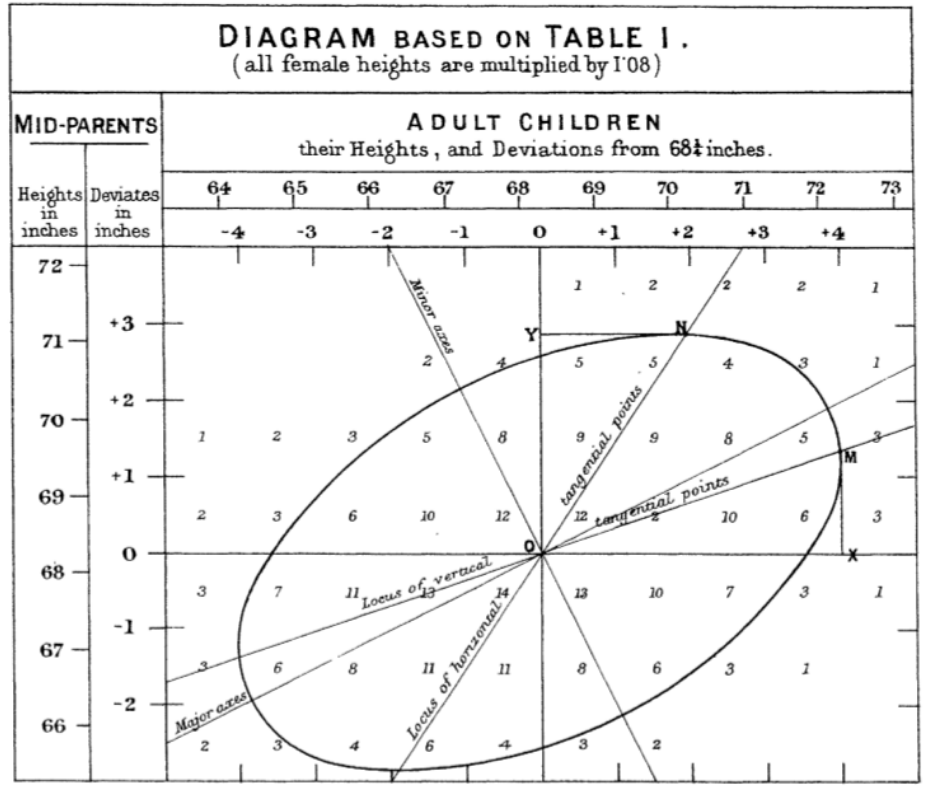
\includegraphics[width=0.7\textwidth]{galton1}
\caption{\label{fig:frog2}\textit{Regresión a la mediocridad de Galton (1889)}.}
\end{figure}

Suponiendo que se quiera predecir el tamaño que un niño tendrá teniendo información de la estatura de los padres, el método de regresión lineal de galton resultaría útil para tal propósito. La información original de Galton se encuentra disponible en algunos paquetes de R. A continuación al ejecutar el código siguiente se obtiene la regresión lineal que estima el tamaño que tendrá alguno de los hijos.

\begin{lstlisting}
## Instalacion de paquetes
install.packages("psych")

## Cargando libreria
library(psych)

## Carga de datos
data("galton")

## Grafica
plot(galton)

## Estimacion del modelo lineal
## Se espefica child = f(parent)
fit <- lm(data = galton, child ~ parent)

## Se grafica la regresion
abline(fit, col = "red", lwd = 3)
\end{lstlisting}


\begin{figure}[H]
\centering
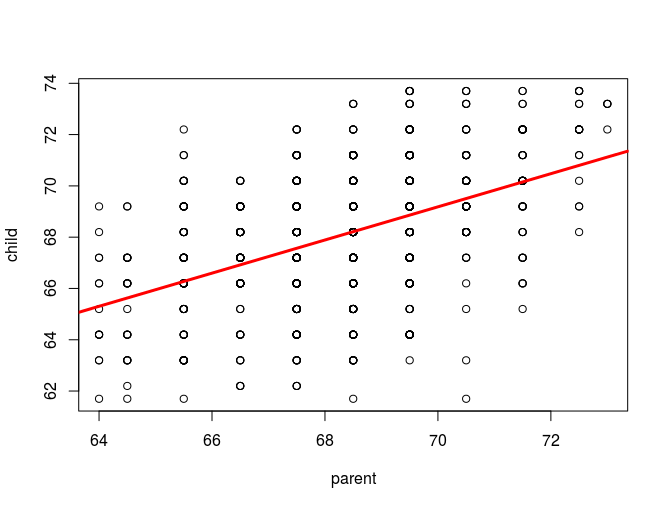
\includegraphics[width=0.7\textwidth]{galton11.png}
\caption{\label{fig:frog2}\textit{Regresión lineal de estatura para padres e hijos en pulgadas. Información de Galton (1889)}.}
\end{figure}


$$ Y = b + mx$$

Una recta que se representa con la ecuación anterior se explica por b que es la ordenada al orígen, m explica la pendiente y x es un valor cualquiera. En el caso del modelo de Galton estimado, la ecuación de la regresión lineal es muy similar.

$$ \hat{Y} = b_0 + b_1 X_i + \epsilon$$

Donde para el modelo de Galton $b_0$ es llamado intercepto y es el símil de la ordenada al origen de la ecuación X, $b_1$ es el coeficiente de X o pendiente m en la ecuación lineal. El siguiente código recrea la ecuación lineal tomando la pendiente (estimador) y ordenada al origen (intercepto) del modelo de regresión de Galton. La figura X muestra gráficamente que la regresión lineal y la recreación utilizando el método de ecuación lineal son iguales.

\begin{lstlisting}
## Estimacion manual del modelo

## Los valores de los coeficientes
fit$coefficients

## Se reconstruyen los valores con la formula
## de ecuacion lineal de la recta
## y = b + mx
recta <-as.numeric(lapply(galton$parent,
                          function(x) fit$coefficients[1] + fit$coefficients[2] * x))

## Se extran los valores del modelo de regresion
original <- fitted.values(fit)

## Graficamos los valores que se predicen y los valores estimados por el modelo
par(mfrow=c(1,2))
s
plot(galton, main = "Modelo de regresion lineal")
lines(galton$parent, original, col = "red", lwd = 3)

plot(galton, main = "Ecuacion de la recta")
lines(galton$parent,recta, col = "blue", lwd = 3)
\end{lstlisting}

\begin{figure}[H]
\centering
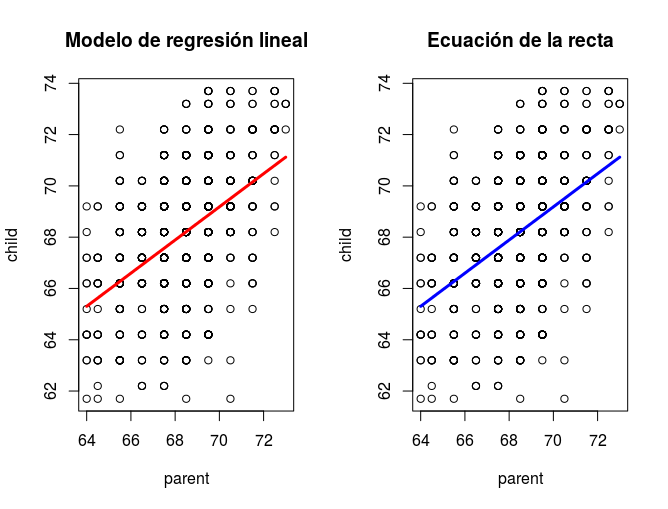
\includegraphics[width=0.7\textwidth]{galton2.png}
\caption{\label{fig:frog2}\textit{Comprobación gráfica de modelo de regresión lineal (izquierda) y estimación por medio de ecuación lineal recta (y = b + mx). Se observa que ambos modelos son iguales para los datos de Galton (1889)}.}
\end{figure}

\section{Clasificación con métodos de regresión lineal}

Ahora se revisa el un caso de clasificación con regresión lineal. Generalmente, para los usos de cotidianos de aprendizaje automatizado se considera la clasificación lineal como una forma sencilla pero poco eficiente para clasificar datos. Un ejemplo claro de ello se puede ver en la figura X. 

La figura muestra que el método de regresión lineal es menos eficiente para clasificar parte de la información que está cercana entre las clases 1 y 3. 

\begin{figure}[H]
\centering
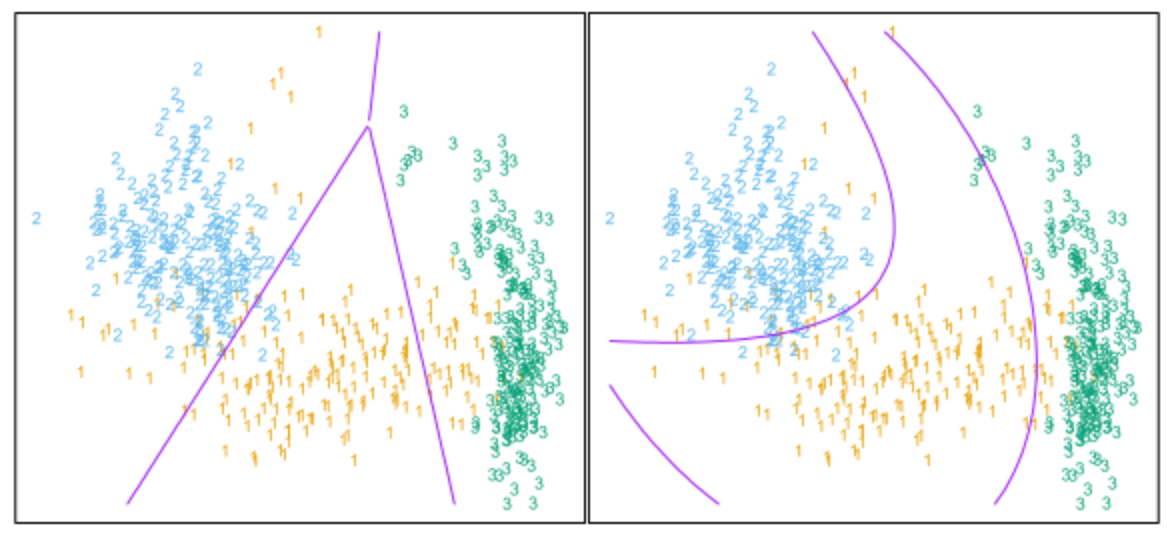
\includegraphics[width=0.7\textwidth]{ng.png}
\caption{\label{fig:frog2}\textit{Dos métodos de clasificación de Hastie (2009). Del lado izquierdo se muestra la clasificación con una función lineal y en el lado derecho una clasificación con una función cuadrática. Se muestra que el modelo de regresión lineal es menos flexible}.}
\end{figure}

Sin embargo, el método de regresión lineal para clasificación es simple pero suficiente para algunos casos. Por ejemplo, la gráfica siguiente un ejercicio simulado muestra un caso de regresión lineal para clasificación, donde las observaciones rojas significan una clase y las categoría negra una clase distinta. De acuerdo con el análisis de clasificación, el método simple de regresión lineal identifica cerca del 70\% de la información adecuadamente. 

\begin{figure}[H]
\centering
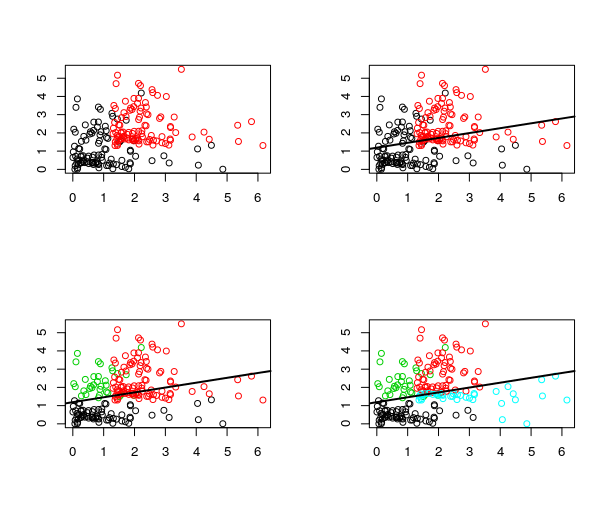
\includegraphics[width=0.7\textwidth]{clasificadorlineal.png}
\caption{\label{fig:frog2}\textit{Modelo de clasificación de regresión lineal aleatorio. Se muestran los pasos en los que se clasifica la información. Las categorías se expresan por colores rojo y negro. Las observaciones clasificadas erróneamente en verde y azul}.}
\end{figure}

Una forma simple de conocer el desempeño de clasificación de un algoritmo, en este caso, el algoritmo de regresión lineal, es contar el número de objetos con una clasificación incorrecta. En el caso de la figura X son todos aquellos puntos negros que se encuentran sobre la línea de regresión y los puntos rojos que están debajo de la línea de regresión. Se suma el número de observaciones con clasificación errónea y se divide entre el número total de observaciones para conocer un tipo de  \textit{misclassification rate}, no es el único método ni el más utilizado, más adelante se revisarán métodos más completos para estimar el poder de clasificación y predicción de un modelo. Para el caso del ejercicio simulado la gráfica muestra los objetos mal clasificados en color verde y azul.

\subsection{Entrenamiento de algoritmo de clasificación lineal}

En un caso tradicional de aprendizaje automatizado, es muy importante buscar relaciones relevantes en la información. El objetivo es tener información suficiente para realizar validaciones de las hipótesis planteadas por alguna clase de algoritmo o modelo que se haya generado. La metodología es simple pero muy eficiente cuando se utiliza de forma correcta. Consiste en tomar una parte de la información que está en un conjunto de datos y utilizarla para crear el modelo. Otra parte de la información servirá para validar el modelo y conocer su poder predictivo. En este caso, se utilizan los principios que un algoritmo de inteligencia artificial tradicional utilizaría en una versión simplificada.

Esta metodología de muestreo para fraccionar la información está especificada a detalle en el capítulo X. Para este caso introductorio, utilizaremos una muestra simple para información de X países y probaremos el modelo de regresión estimado para X países. 

A continuación se utiliza el método de regresión lineal para clasificar un caso con información real. El objetivo de este modelo simple es segmentar aquellos países pertenecientes a la OCDE y aquellos países que no pertenecen a este grupo. Los alcances de este ejercicio son muy amplios, aunque en este apartado se enfoca en desarrollar un modelo que ayude a clasificar información nueva en función del modelo previo. 

En general, este simple algoritmo de aprendizaje automatizado nos dará la capacidad de enseñar un modelo estadístico a nuestro primer sistema de inteligencia artificial a clasificar información en función a una \textit{fase de entrenamiento}. En esta \textit{fase de entrenamiento} se establece el modelo de regresión lineal determina si un país pertenece a la OCDE en función de dos variable simples. Se toman como variables dos focos importantes para el desarrollo según las métricas del banco mundial. En la figura X se observa el modelo de clasificación para la muestra de entrenamiento en 58 países.

\begin{lstlisting}
### Clasificador de paises OCDE

## Entrenamiento

## Lectura del archivo de entrenamiento
df <- read.csv(file = "Cap 1. Principios de aprendizaje automatizado/data_countries.csv")

## Se observan las variables
names(df)

## Cambiando los nombres de todas las variables
## se utiliza una lista de nombres mas sencilla de interpretar

names(df) <- c("Nombre_pais",
               "Codigo_pais",
               "Tasa_mortalidad",
               "GNI_PC_PPP",
               "OCDE_member")

## Grafica de dispersion de los datos seleccionados, sin distincion por clase
par(mfrow=c(1,2)) ## Se especifica que se quieren dos graficas en un mismo renglon

## Grafica 1 de 2 Mortalidad infantil e ingres nacional bruto.
plot(x = df$Tasa_mortalidad,  ## Variable X
     y = df$GNI_PC_PPP,       ## Variable Y
     xlab = "Tasa de Mortalidad infantil por cada mil nacimientos (2015)",
     ylab = "Ingreso Nacional Bruto precios corrientes PPP (2015) ")


## Estimacion del modelo de regresion lineal.
## se especifica que el ingreso nacional bruto = f(Tasa de mortalidad)
## la variable Y del modelo es ingreso nacional bruto
## la variable X del modelo es Tasa de mortalidad

a <- lm(data = df,  GNI_PC_PPP ~ Tasa_mortalidad)

## Se pintan los casos que estan mal clasificados
df$OCDE_member[df$Tasa_mortalidad > 75] <- 3

## Grafica 2 de 2 Mortalidad infantil e ingres nacional bruto, colores por clasificacion de pais
plot(df$Tasa_mortalidad,
     df$GNI_PC_PPP, col = df$OCDE,
     xlab = "Tasa de Mortalidad infantil por cada mil nacimientos (2015)",
     ylab = "Ingreso Nacional Bruto precios corrientes PPP (2015) ")

abline(a, col = "blue", lwd = 3)
\end{lstlisting}

\begin{figure}[H]
\centering
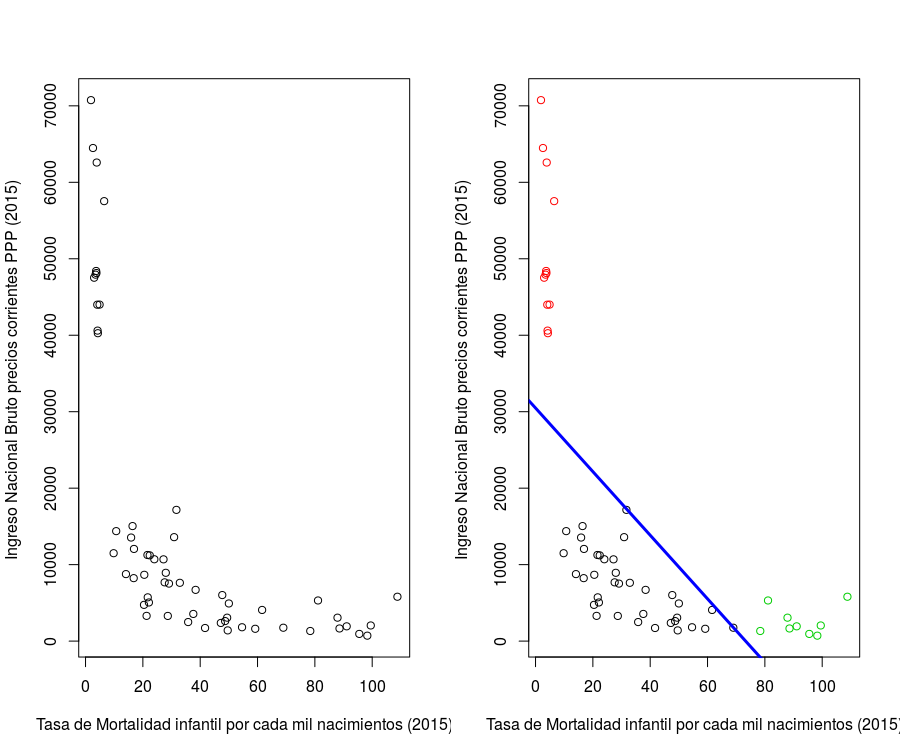
\includegraphics[width=0.7\textwidth]{clasificadorlinealentrenamiento.png}
\caption{\label{fig:frog2}\textit{Estimación de modelo de clasificación de países que pertenecen a la OCDE en el set de entrenamiento. Del lado izquierdo se muestra la información para una muestra de 58 países. En el lado izquierdo se observa el modelo de regresión lineal y la información según su categoría. En rojo se observan los países que pertenecen a la OCDE, en negro aquellos que no pertenecen y en verde son los errores de clasificación}.}
\end{figure}

Se segmentan los países con el método de regresión lineal y se obtiene el resultado del modelo clasificatorio. En la figura X del lado izquierdo se observan los datos de Ingreso Nacional Bruto y la tasa de mortalidad por país de la muestra de entrenamiento. Del lado derecho se pinta la información según la clase a la que pertenece. Los países de color rojo corresponden a naciones pertenecientes a la OCDE y de color negro aquellas que no. Según el modelo de clasificación de regresión lineal estimado los países de color verde están clasificados de forma incorrecta. Para el algoritmo planteado, representan errores de clasificación que demuestran el desempeño del sistema inteligente. 

\subsection{Prueba del algoritmo de clasificación lineal}


El modelo anterior clasifica adecuadamente el 84\% de las observaciones en la \textit{fase de entrenamiento} y el  16\% error se concentra en asignar países que no pertenecen a la OCDE. Los errores de clasificación se muestran en color verde y los aciertos en color rojo.

Una vez que el modelo muestra cierta capacidad de clasificación, se procede a hacer las pruebas con el resto de la información. La sección de los datos que se utiliza para la validación de los algoritmos se llama \textit{fase de prueba} y siempre es posterior a la \textit{fase de entrenamiento}. Adicionalmente a estas dos fases, en muchos casos es recomendable utilizar una fase intermedia que se llama \textit{fase de validación}.

Para este caso, el set de prueba se compone del resto de países. Se toma el mismo modelo de regresión lineal que se utilizó para el set de entrenamiento y se observa el desempeño clasificatorio con la información completa. En la figura X se muestran el resultado del modelo de regresión para cerca de 200 países.

\begin{lstlisting}
## Clasificador para todos los paises

#install.packages("dplyr") ## libreria basica de manejo de datos
library(dplyr) ## se carga la libreria

## Juntando bases de datos para flag OCDE
A <- read.csv(file = "Cap 1. Principios de aprendizaje automatizado/data/all_contries.csv",
              stringsAsFactors = F)

B <- read.csv(file = "Cap 1. Principios de aprendizaje automatizado/data/ocde_members.csv",
             stringsAsFactors = F) %>% select(-Date)

df2 <- left_join(A, B)

## Se pintan los casos que no son miembros de la OCDE con color 1 (negro)
df2$OCDE_member[is.na(df2$OCDE_member)] <- 1


## Cambiando los nombres de todas las variables
## se utiliza una lista de nombres mas sencilla de interpretar
names(df2) <-c("Nombre_pais",
               "Codigo_pais",
               "GNI_PC_PPP",
               "Tasa_mortalidad",
               "OCDE_member")
df2$OCDE_member[df2$Nombre_pais == "World"] <- 3


par(mfrow=c(1,1))
plot(df2$Tasa_mortalidad,
     df2$GNI_PC_PPP,
     col = df2$OCDE_member,
     xlab = "Tasa de Mortalidad infantil por cada mil nacimientos (2015)",
     ylab = "Ingreso Nacional Bruto precios corrientes PPP (2015) ")
abline(a, col = "blue", lwd = 3)
\end{lstlisting}

\begin{figure}[H]
\centering
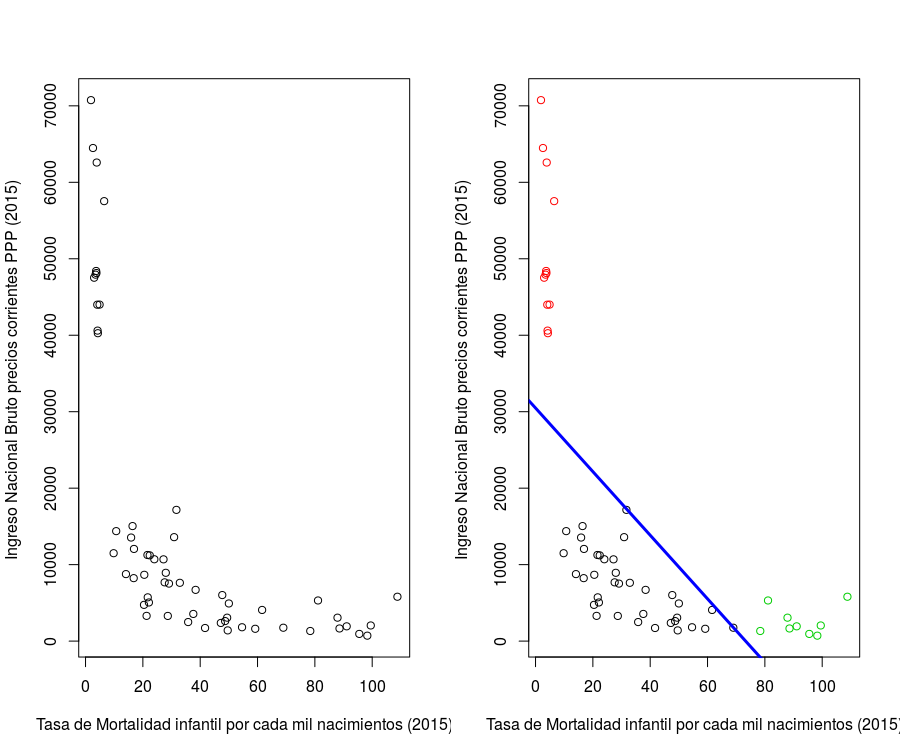
\includegraphics[width=0.7\textwidth]{clasificadorlinealentrenamiento.png}
\caption{\label{fig:frog2}\textit{Estimación de modelo de regresión lineal. Clasificación de países que pertenecen a la OCDE en el set de prueba. En color rojo se observan países que pertenecen a la OCDE y en negro países que no pertenecen a esta organización}.}
\end{figure}

Es importante destacar que se utiliza el mismo modelo de regresión que se presenta en la figura X - 1, no se vuelve a crear un modelo aunque la información haya cambiado. Para la mayoría de los casos, el set de prueba tiene un desempeño menor que el set de entrenamiento. Para el caso de los países de pertenecientes a la OCDE el desempeño de 77\% de los casos clasificados correctamente es menor, el porcentaje de error se considera aceptable. 

El modelo de regresión lineal estimado resulta útil para clasificar la información. A pesar de la simpleza del modelo, es bastante más eficiente que una elección aleatoria. Comparar el desempeño del modelo con una selección aleatoria es una forma popular de identificar si el modelo contribuyó a clasificar mejor o no. Una elección aleatoria se define como la probabilidad simple de elegir un objeto x o y, según sea el caso.\footnote{Por ejemplo, si se tiene una caja con 6 pelotas color rojo y 4 pelotas color blanco la probabilidad simple de elegir una pelota roja es del 60\% y un 40\% de elegir una pelota de color blanco. Un modelo de clasificación adecuado debe tener un desempeño mayor que una probabilidad simple. Suponiendo que sabemos que las pelotas rojas se concentran más del lado izquierdo, un criterio ejemplo, sería siempre elegir las pelotas que están del lado izquierdo, de esta manera la probabilidad de elegir una pelota roja es del 80\% por ejemplo.} Mediante una elección aleatoria se puede de conocer si el modelo es útil o es menos eficiente que una elección al azar.  Para este caso en concreto, si se utiliza el método aleatorio la probabilidad de elegir un país de la OCDE de toda la muestra es de cerca del 16\% y de un 37\% si se utiliza el algoritmo de regresión lineal propuesto, por lo tanto, el método de clasificación de regresión lineal ayuda a hacer una elección 2.3 veces más precisa.

Para una estimación más avanzada del desempeño del algoritmo,  generalmente se utiliza el bayes error rate o error bayesiano que estima la probabilidad de error para algoritmos de de clasificación. En las secciones por venir se revisan distintos métodos para comparar el desempeño de un algoritmo.

Finalmente, el algoritmo de clasificación está terminado. Con un buen desempeño para los datos anteriores, el algoritmo se puede utilizar para comenzar a clasificar información. Podría funcionar como una clase (muy simple pero eficiente) de inteligencia artificial. Por ejemplo, si conocemos el ingreso bruto de una región específica y los índices de mortalidad infantil, podremos utilizar el algoritmo para analizar si el desarrollo económico de la región podría pertenecer a los estándares de un país perteneciente a la OCDE. El la figura siguiente se presenta un caso similar. 

Finalmente, el algoritmo de clasificación está terminado. Con un buen desempeño para los datos anteriores, el algoritmo se puede utilizar para comenzar a clasificar información. Podría funcionar como una clase (muy simple pero eficiente) de inteligencia artificial. Por ejemplo, si conocemos el ingreso bruto de una región específica y los índices de mortalidad infantil, podremos utilizar el algoritmo para analizar si el desarrollo económico de la región podría pertenecer a los estándares de un país perteneciente a la OCDE. El la figura siguiente se presenta un caso similar. 

\begin{lstlisting}
x <- c(5, 7, 9)
y <- c(17000, 70000,32000)
p<- data.frame(x, y)

## Se pintan los puntos al grafico anterior
points(p, col = "cyan", lwd = 10)

a$coefficients <- a$coefficients * -2
abline(a, col = "blue", lwd = 3 )

a$coefficients <- abs(a$coefficients) + 100
abline(a, col = "blue", lwd = 3 )
\end{lstlisting}

\begin{figure}[H]
\centering
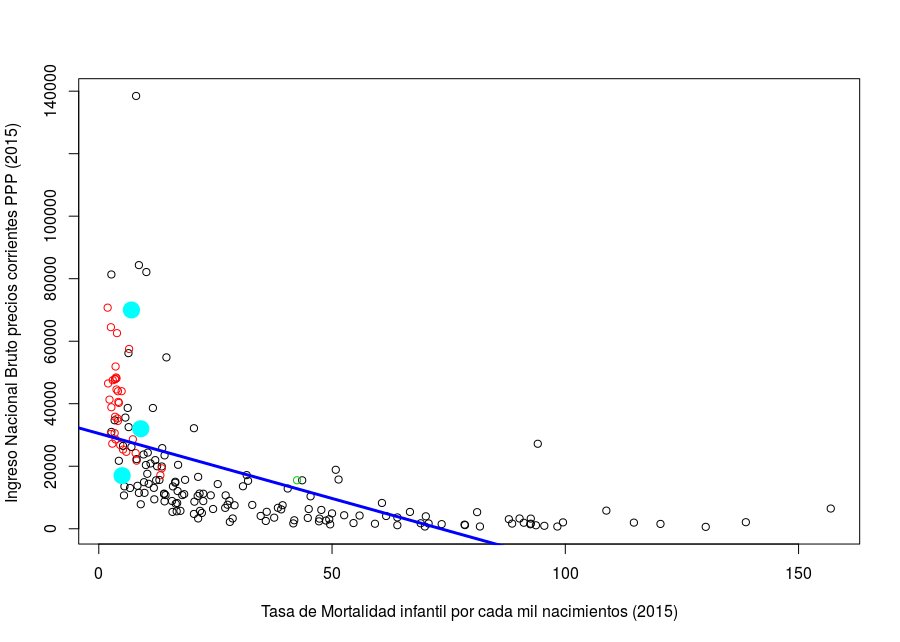
\includegraphics[width=0.7\textwidth]{clasificadorlinealnuevos.png}
\caption{\label{fig:frog2}\textit{}}
\end{figure}

En la figura anterior se tienen 3 regiones nuevas que son clasificadas por el algoritmo lineal, de acuerdo el modelo de clasificación se obtiene que dos de ellos con alta probabilidad tienen las condiciones que priman en un país que pertenece a la OCDE y aquel que se encuentra debajo de la línea de regresión no lo es. 

Supongamos para medición de desigualdad en una nación latinoamericana se comparan los estándares de vida de una región con acceso restringido a la salud y regiones de alto ingreso económico que son aledañas. Posiblemente las regiones de alto ingreso económico tendrán estándares de vida similares a países pertenecientes a la OCDE y las aledañas no tendrán estos estándares de vida. Rápidamente, este modelo nos ayudará a determinar los límites en función a información de mortalidad infantil e ingreso nacional; posibles medidas de política económica u objetivos de política social.

\textit{¡Felicidades, si has seguido todos los pasos de esta sección exitosamente has creado un primer algoritmo simplificado de inteligencia artificial! Tu nuevo algoritmo te permitirá tomar decisiones de política económica y social.}

Con el fin de reforzar las habilidades de modelización presentadas en esta sección introductoria, más adelante se revisarán a detalle algunos algoritmos más avanzados de clasificación y predicción. Igualmente, se explicarán las metodologías estándar de muestreo así como pruebas de validación de los modelos de aprendizaje automático. En el capítulo siguiente se muestra el algoritmo de agrupamiento o cluster por LDA (\textit{Linear Discriminant Analysis} por sus siglas en inglés) y una aplicación relacionada a optimización de centros de distribución con una perspectiva geográfica.

\subsection{Resumen}

ste capítulo se enfoca en desarrollar los conceptos clave de regresión lineal aplicados a un sistema de aprendizaje automático simplificado. Se revisan los conceptos del modelo de regresión lineal, así mismo, se explica que el modelo de regresión lineal tiene un origen más antiguo de lo que comúnmente se puede creer y se explican los planteamientos que desarrolló Francis Galton en el siglo XIX para llegar a las conclusiones de que existe un modelo de regresión lineal. 

Adicionalmente, se demuestra la similitud que tiene la regresión lineal con la ecuación simple de la recta ($y =mx * b$), con el fin de comprender las funciones de los estimadores y coeficientes en un modelo de regresión lineal. Mediante una explicación práctica en R, se utiliza un modelo de regresión lineal propio para recrear las investigaciones de Galton (1889). 

Posteriormente se muestra el proceso gráfico de clasificación lineal con información aleatoria y más adelante, se revisa el uso del modelo de regresión lineal para problemas de clasificación con información real. Se especifica que la clasificación es un tema fundamental en inteligencia artificial y machine learning o aprendizaje automático. Por medio de los principios básicos de regresión lineal, se ejecutan todos los pasos básicos para crear un sistema de inteligencia artificial simple aplicado a un problema económico. 

Se utilizan las metodologías tradicionales de machine learning de muestreo, entrenamiento y prueba para ejemplificar el caso de clasificación de la OCDE y se muestra el funcionamiento. El modelo pretende aprender clasificar países que pertenecen a la OCDE (reconocidos por ser países desarrollados y algunos en vías de desarrollo) y aquellos que no pertenecen a la OCDE. Se utilizan datos del banco mundial tomando métricas clave para el desarrollo y se entrena el modelo de regresión lineal con un poder de clasificación adecuado. 


\chapter{Algoritmos de clasificación lineal}

\begin{flushright}
\textit{“Admittedly, no Artificial Intelligence economic forecasting system is operational today, while econometric approaches have the very real merit of existing. However, several experiments have yielded encouraging results and posed useful and pertinent questions. Is econometrics a satisfactory representation of the world? Are the limitations on the models nothing more than superficial defects due to the inadequacies of existing technology?”}

Palies, O y Mayer,  J (1989)
\end{flushright}

En esta sección se revisan dos métodos populares de clasificación. Los algoritmos de clasificación tienen como objetivo segmentar e identificar información. En la primera sección, se revisaron los principios básicos que todo sistema de inteligencia artificial soluciona, la diferencia entre un algoritmo supervisado y no supervisado, así como una aplicación simple con modelos de regresión lineal para clasificar datos. Para este apartado, se encuentran explicados un par de métodos de clasificación muy comunes que sugieren bases para implementaciones más complejas. El objetivo de esta sección es complementar el uso del método de regresión lineal y ser aprovechado en un contexto más extenso que permita identificar clusters supervisados. Siguiendo el objetivo de este texto, se presenta una visión práctica de los algoritmos. 

Las aplicaciones de este tipo de algoritmos son recurrentes en ramas de la ciencia como biología o ingeniería. Diversos estudios utilizan estos métodos para identificar patrones en comportamiento en seguridad de sistemas, tráfico de redes e identificación de factores que pueden predecir riesgo de enfermedades en una población. Inclusive, algunos especialistas en bioestadística identifican patrones dentro del ADN para detectar las causas genéticas de enfermedades o encontrar grupos de especies (Hoang et al, 2015). Algunos de las técnicas de clasificación o identificación de clusters se utilizan frecuentemente para identificar ataques a servidores corporativos y gubernamentales (Aghabozorgi et al, 2015). Algunas ramas toman este tipo de algoritmos para clasificar la intención de un texto o comando de voz de forma automática.

Usualmente, las técnicas de cluster no forman parte de las herramientas tradicionales que un científico social desarrolla. En caso de la Economía, un texto de econometría tradicional difícilmente incluirá estas técnicas como argumento principal del libro. Aunque varias investigaciones de clusters industriales, de mercados financieros e internacionales utilizan estas técnicas resultan trabajos de desarrollos técnicos y estadísticos más avanzados. Sin embargo, este no es el caso para las demás disciplinas. Por ejemplo, que dentro de las ciencias sociales estas metodologías no son ajenas a investigaciones relacionadas con identificación de espacios geográficos o identificación de grupos en torno a análisis espacial y todas las vertientes interdisciplinarias. En marketing, los análisis de cluster resultan fundamentales para identificar grupos objetivos para hacer más eficientes las campañas de publicidad. En esta rama las aplicaciones de clúster se han madurado enormemente en análisis de redes sociales de \textit{Facebook}, \textit{Twitter} y Yelp por ejemplo.

Los algoritmos de clustering son generalmente utilizados por aquellos que manejan las ramas de inteligencia artificial machine learning y data mining. Algunos algoritmos de clustering no son técnicas nuevas y generalmente se les atribuye como técnicas de aprendizaje no supervisado. Según se definió en la primera sección del texto el aprendizaje no supervisado se caracteriza por no tener conocimiento a priori de las categorías que componen una muestra. Los objetivos de un modelo de clustering son caracterizados por segmentar e identificar estas clases o categorías.\footnote{Algunos autores mencionan que los objetivos de clustering pueden ser distintos, por ejemplo Wu (2012) menciona que los propósitos de un algoritmo de agrupamiento es entender características en los datos y ser utilizado como muestras prototipo.} Un ejemplo interesante de clustering se puede ver en los vehículos de conducción autónoma de Tesla. En el siguiente vínculo se puede ver que en tiempo real el automóvil identifica al menos siete clases distintas. 

\begin{enumerate}
\item \textit{Motionflow}
\item \textit{Lane lines}
\item\textit{Road FLow}
\item \textit{In path objects}
\item \textit{Road lights}
\item \textit{Objects}
\item \textit{Road signs}
\end{enumerate}

\begin{figure}[H]
\centering
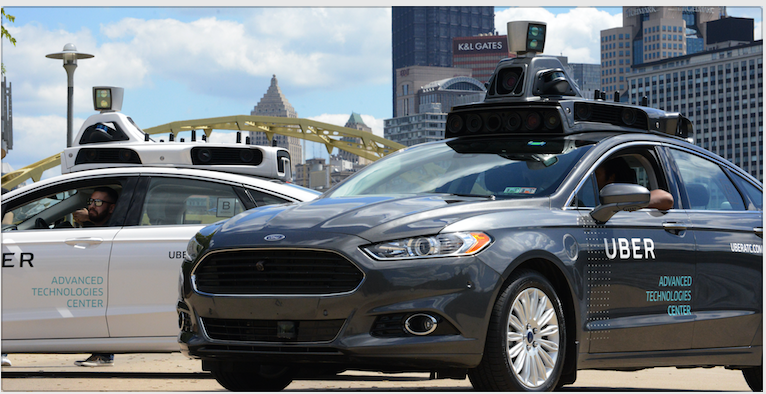
\includegraphics[width=0.9\textwidth]{uber1.png}
\caption{\label{fig:frog2}\textit{Vehículo de conducción asistida de Uber. \url{https://www.youtube.com/watch?v=VG68SKoG7vE}}}
\end{figure}

Esta sección se enfoca en mostrar aplicaciones de un algoritmo de clustering similar a los casos que se describen anteriormente. Se busca encontrar grupos en información clasificada y no clasificada utilizando una técnica popular conocida como \textit{Linear Discriminant Analysis} (LDA) se analizará un caso muy popular de “taxonomía” en biología para conocer los principios del análisis y un caso campaña de marketing para identificar grupos de clientes potenciales.

\subsection{Clasificación de múltiples categorías con análisis discriminante lineal (LDA)}

El orígen de la popular técnica de aprendizaje estadístico LDA se encuentra en uno de los artículos más relevantes de la estadística moderna The use of multiple measurements in taxonomic problems de Fisher en 1936, famoso biólogo y estadístico es conocido por sus aportes a las ciencias naturales y a la inferencia estadística. La taxonomía es conocida como la ciencia de la clasificación y Fisher tenía como objetivo encontrar un método estadístico que pudiera maximizar la diferencia entre las cuatro clases de flores que estaba analizando, es decir, mostrar más facilmente las diferencias entre especies, en esencia un problema de clasificación o taxonomía. Aunque el método presentado por Fisher en el artículo original es útil para clasificar información, se utilizan los datos originales de FIsher y el método generalizado para k clases de LDA. Usualmente, se atribuye que el método de LDA es la versión generalizada del método original de Fisher y por lo tanto más adecuado para una clasificación de k clases.\footnote{Otras variantes de clasificación pueden ser los modelos logit y probit que se abordan en gran parte los textos convencionales de econometría, por ejemplo:  Gujarati (2012).}

A continuación, utilizaremos el método de LDA para clasificar los mismos datos que recolectó Fisher en 1936. De acuerdo con la información se tienen tres tipos distintos de especies\textit{ Iris setosa, Iris versicolor, Iris virginica.} En la figura X se observa a simple vista cierta similitud de color entre las especies de Iris y resulta un reto interesante poder diferenciar cada una de ellas según ciertas características.

\begin{figure}[H]
\centering
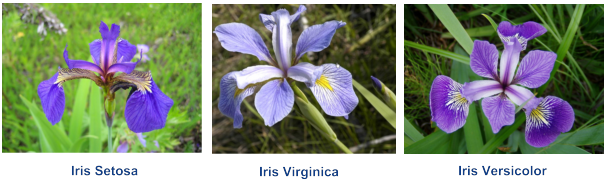
\includegraphics[width=1\textwidth]{iris1.png}
\caption{\label{fig:frog2}\textit{Se muestran las 3 especies que componen los datos de Fisher 1936.}}
\end{figure}

Fisher originalmente utiliza cuatro distintas características cuantitativas de estas especies, el largo del pétalo, ancho del pétalo, largo del sépalo y ancho del sépalo. La función principal de un sépalo es cubrir los pétalos y otras piezas florales en etapas primitivas de desarrollo de una flor. Para una flor de género Ludwigia se observa claramente la diferencia entre pétalo y sépalo.

A continuación se muestran algunos de los ejemplos que compone la información recolectada por Fisher. Se muestran las 4 categorías que caracterizan a cada una de las flores medidas en cm y a la especie a la que pertenece (setosa, virginica o versicolor). Según los criterios que se definieron en la sección 1 del texto, este caso es característico de un problema de segmentación clasificado o aprendizaje supervisado. Al conocer la clase a la que pertenece cada flor se puede ejecutar un algoritmo que tome en cuenta esta variable supervisada (Species).

Para explorar y mostrar la diferencia en cada una de las especies, se grafican las 150 muestras para las cinco dimensiones descritas. En la figura X se explica la dispersión por variable y por color de especie. 

\begin{lstlisting}
## Se carga la informacion
df <- iris

## Se describen las primeras lineas de los datos
head(df)

\end{lstlisting}

\begin{figure}[H]
\centering
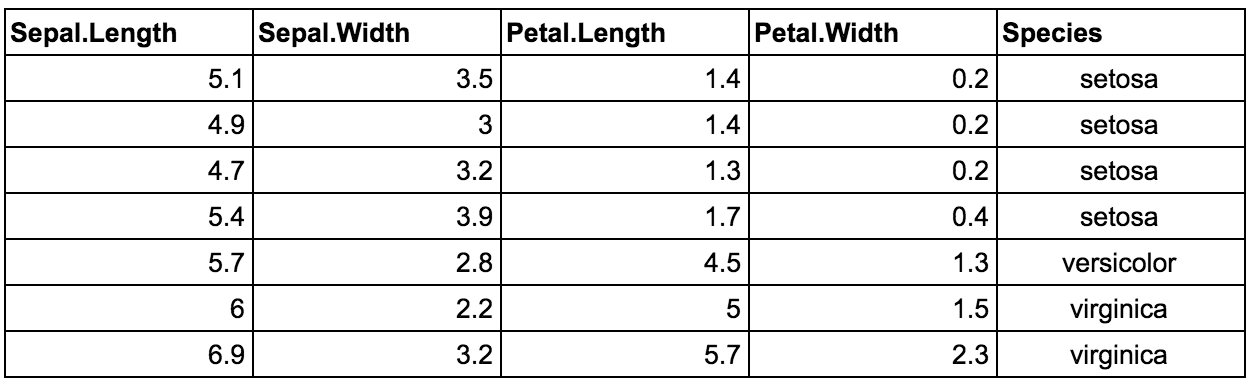
\includegraphics[width=1\textwidth]{iris2.png}
\caption{\label{fig:frog2}\textit{Selección aleatoria de la información recolectada por Fisher 1936. Se observan las 4 características de las flores y la especie a la que pertenecen. }}
\end{figure}

\begin{lstlisting}
## Se grafican las 5 dimensiones de la informacion
## se colorea segun la especie a la que pertenece cada flor

plot(df, col = df$Species)
\end{lstlisting}

\begin{figure}[H]
\centering
\includegraphics[width=1\textwidth]{iris3.png}
\caption{\label{fig:frog2}\textit{Gráfica de dispersión para las cinco dimensiones de Fisher (1936). En color negro se muestran iris setosa, en rojo iris versicolor y en color verde iris virginica. }}
\end{figure}

A simple vista se observa que una posible decisión para identificar la clase iris setosa (negro) son todas aquellas muestras que tengan menos de 2.5cm de largo en el pétalo y menos de 6cm de largo en el sépalo. Sin embargo, la regla de segmentación para el caso de las especies iris versicolor e iris virginica no es tan evidente (rojo y verde respectivamente). Al elegir una regla arbitraria de discriminación (línea azul) no se clasifican correctamente algunas observaciones.

\begin{figure}[H]
\centering
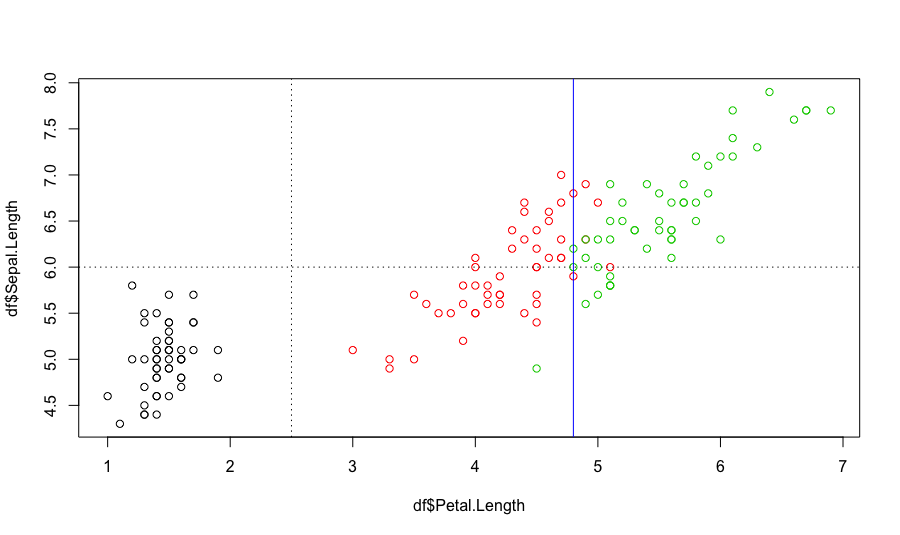
\includegraphics[width=1\textwidth]{iris4.png}
\caption{\label{fig:frog2}\textit{Gráfica de dispersión para las cinco dimensiones de Fisher (1936). En color negro se muestran iris setosa, en rojo iris versicolor y en color verde iris virginica. }}
\end{figure}

Puesto que las reglas arbitrarias no representan un método riguroso de análisis, utilizando el método de LDA generalizado se pueden clasificar las especies. Para ejecutar el método de forma adecuada generalmente se utilizan técnicas de muestreo aleatorio antes de ejecutar el algoritmo de LDA. La relevancia de un muestreo adecuado impactará el desempeño de cualquier modelo de segmentación, identificación y predicción. Para cualquier análisis de machine learning el muestreo representa las bases que permitirán efectuar y ajustar un algoritmo de forma adecuada. 

A continuación se describe una técnica de muestreo común en las ciencias computacionales. Consiste en dividir la información en set de pruebas y set de validación. En la sección primera de este texto se menciona el uso de esta técnica, en el siguiente apartado se revisa con un poco más de profundidad.

\subsection{Fase de entrenamiento}

La sección de entrenamiento o \textit{training set}, consiste en una sección de la información que será utilizada para entrenar el modelo de segmentación. Una forma simple es utilizar una selección aleatoria de una porción determinada de la información, así por ejemplo, se utiliza una porción significativa de los datos para estimar el modelo. Esta técnica permite entrenar el modelo en una sección de los datos y validarlo en otra sección generalmente más pequeña. En la figura X se explica cómo se divide la información para el caso de las especies iris. Se tienen 150 observaciones que constituye la población, se toma aleatoriamente el 70\% para entrenar el modelo en la fase de entrenamiento y el 30\% restante se seleccionan para la fase de pruebas.

\begin{figure}[H]
\centering
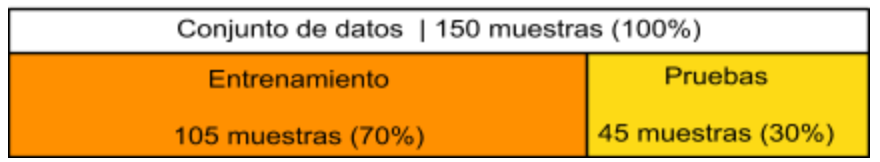
\includegraphics[width=1\textwidth]{fase1.png}
\caption{\label{fig:frog2}\textit{Esquema de muestreo aleatorio para el caso de iris. Se muestran el número de observaciones que se utilizan por fases según el entrenamiento y prueba del algoritmo.}}
\end{figure}

\begin{lstlisting}
## Fase de entrenamiento
## Seleccion del 70% de la informacion

porcentaje <- 70/100

num_muestras <- porcentaje * nrow(df)

## Muestreo aleatorio
set.seed(20)
train_ind <- sample(seq_len(nrow(df)), size = num_muestras)

## Seleccionamos las muestras que pertenecen
## al set de entrenamiento
train_set <- df[train_ind, ]

## Seleccionamos el resto de muestras
## que pertenecen al set de pruebas
test_set <- df[-train_ind, ]
\end{lstlisting}

Al seleccionar el dataset de entrenamiento train\_set observamos las probabilidades a priori que describen la probabilidad simple de elegir una clase de forma aleatoria. A continuación se muestran las probabilidades a priori para cada una de las especies así como el número de veces que aparece cada clase en la muestra de 105 observaciones.

\begin{lstlisting}
## Ejecucion del algoritmo de LDA

library(MASS)
source(file = 'Cap 2. Algoritmos de clasificacion lineal/diferencias_iris.R')


## Ejecucion del algoritmo de LDA
modelo <- lda(data =train_set, Species ~.)


## Probabilidades a priori
modelo$prior

## Numero de observaciones por clase
modelo$counts

## Coeficientes por caracteristicas
modelo$scaling
\end{lstlisting}

\begin{figure}[H]
\centering
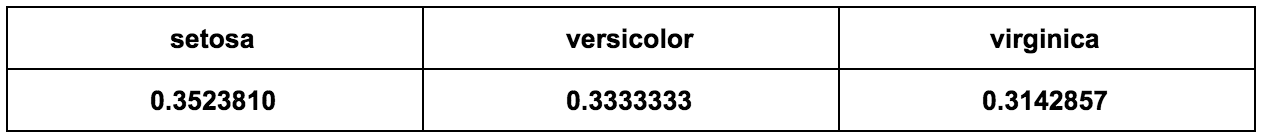
\includegraphics[width=1\textwidth]{fase2.png}
\caption{\label{fig:frog2}\textit{Probabilidades a priori del modelo LDA para todas las clases para el set de entrenamiento.}}
\end{figure}

\begin{figure}[H]
\centering
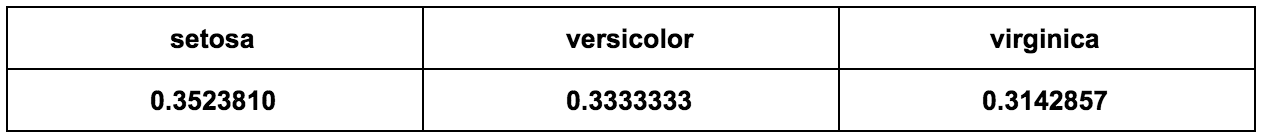
\includegraphics[width=1\textwidth]{fase2.png}
\caption{\label{fig:frog2}\textit{Número de observaciones por clase para el set de entrenamiento.}}
\end{figure}

Las tablas anteriores nos describen la probabilidad de obtener una clase u otra según la probabilidad simple. Recordemos que al tener información a priori del conjunto de información que se quiere clasificar se está hablando de un algoritmo supervisado. En función a estos valores el algoritmo de LDA creará las reglas de decisión para clasificar los datos en función de sus características, \textit{sepal length, sepal width, petal length y petal width}. Las reglas de decisión se caracterizan por cada una de una estas 4 variables en un plano bidimensional; es decir, cada característica tendrá reglas de decisión para dos dimensiones.

\begin{figure}[H]
\centering
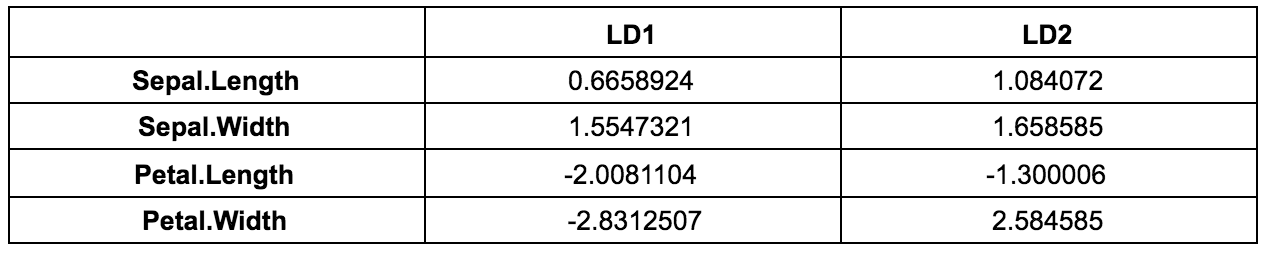
\includegraphics[width=1\textwidth]{fase4.png}
\caption{\label{fig:frog2}\textit{Coeficientes del modelo LDA}}
\end{figure}

\begin{lstlisting}
## Se predice el modelo sobre el set  de entrenamiento, por default 
## no se especifica un dataset nuevo a la funcion predict

prediccion <- predict(modelo)

## Grafica de clasificacion original
par(mfrow=c(1,2))
plot(prediccion$x, 
     col =train_set$Species,
     main = "Original")

## Grafica de clasificacion segun el modelo estimado
plot(prediccion$x, 
     col =prediccion$class,
     main = "Prediccion")
\end{lstlisting}

\begin{figure}[H]
\centering
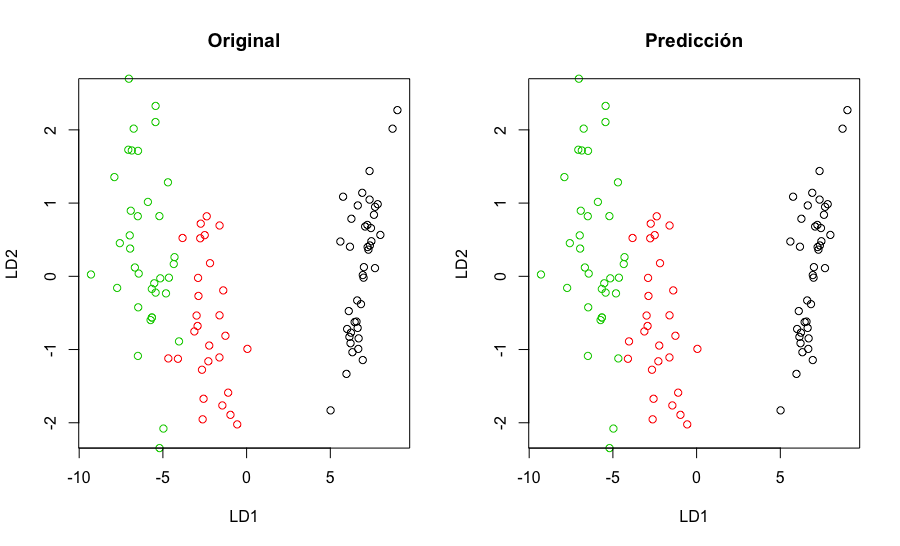
\includegraphics[width=1\textwidth]{fase5.png}
\caption{\label{fig:frog2}\textit{Resultados del modelo de clasificación para los datos de Fisher (1936). Del lado izquierdo se muestra la clasificación original o real por objeto. Del lado derecho las predicciones por el algoritmo de LDA generalizado.}}
\end{figure}

A simple vista en la figura anterior se muestra que el algoritmo de clasificación LDA tiene un desempeño aceptable, del lado izquierdo se muestra la clasificación real por especie y del lado derecho se muestra la clasificación efectuada por el modelo propuesto. A continuación se analiza el desempeño de clasificación real. 

Un ejemplo sería tratar de clasificar el sexo de un paciente según  su estatura, supongamos que tenemos 10 pacientes, 5 que son hombres y 5 que son mujeres. De acuerdo con su estatura creamos un algoritmo que nos dice lo siguiente.

\begin{figure}[H]
\centering
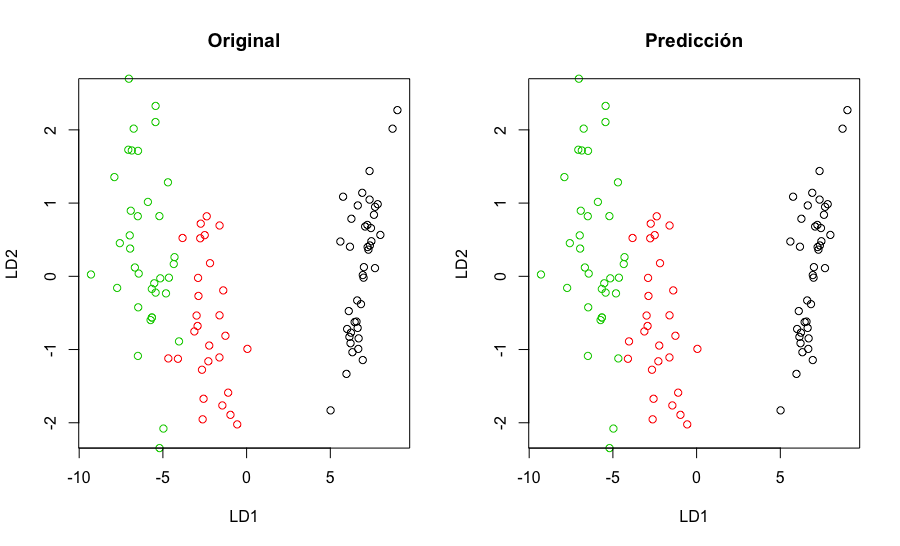
\includegraphics[width=1\textwidth]{fase5.png}
\caption{\label{fig:frog2}\textit{Resultados del modelo de clasificación para los datos de Fisher (1936). Del lado izquierdo se muestra la clasificación original o real por objeto. Del lado derecho las predicciones por el algoritmo de LDA generalizado.}}
\end{figure}

\subsection{Un método de medición del desempeño supervisado}

Un método tradicional utilizado en diversas ramas de la inteligencia artificial para conocer el desempeño de un algoritmo de clasificación y predicción es conocido como matriz de confusión. La matriz de confusión es característica esencial para todo problema de clasificación supervisado. El objetivo de este método es especificar el número de errores en los que incurre el modelo diseñado comparándolo con la información real.\footnote{ Una explicación más completa de esta herramienta de machine learning puede encontrarse en Hastie (2009), y Murphy (2012). En este apartado introductorio las cuestiones de desempeño por especificidad y sensibilidad no son explicadas a detalle.}

\begin{figure}[H]
\centering
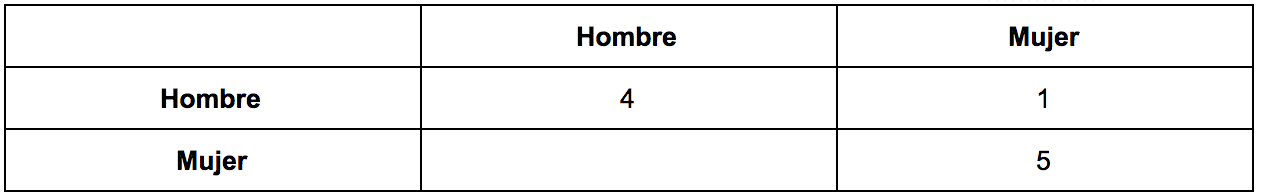
\includegraphics[width=1\textwidth]{fase6.png}
\caption{\label{fig:frog2}\textit{Ejemplo de matriz de confusión, se muestran los verdaderos positivos y verdaderos negativos en la diagonal, falsos positivos y falsos negativos fuera de ella. El modelo predice erróneamente a un hombre como mujer (se muestra fuera de la diagonal. }}
\end{figure}

En el ejemplo hipotético anterior el modelo es bueno identificando mujeres según su estatura al predecir las 5 mujeres como mujeres sin embargo no es tan bueno identificando a todos los hombres, la matriz de confusión explica que un hombre fue catalogado como mujer según sus características.

En el caso de iris, se tiene un modelo para 105 muestras de 150 datos. Se clasificaron las 105 muestras como se observa en la figura anterior y se obtuvieron los resultados del modelo. Para corroborar que el modelo es adecuado, se muestra la matriz de confusión para el set de entrenamiento de la siguiente forma.

\begin{lstlisting}
## Matriz de confusion
## Se muestran las clasificaciones correctas
## en la diagonal

table(prediccion$class, train_set$Species)
\end{lstlisting}

\begin{figure}[H]
\centering
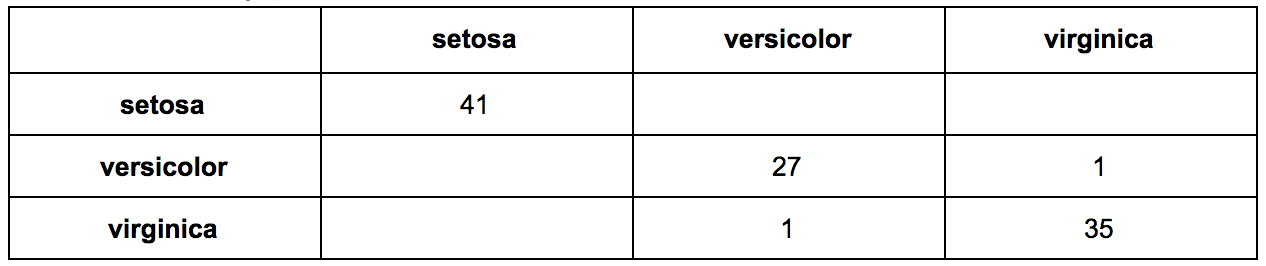
\includegraphics[width=1\textwidth]{fase7.png}
\caption{\label{fig:frog2}\textit{Matriz de confusión para el set de entrenamiento.}}
\end{figure}

De acuerdo con la matriz de confusión, se observan 2 casos erróneos (fuera de la diagonal). Para este caso se muestra que el modelo logra clasificar 98\% de los casos correctamente y el 2\% erróneo corresponde a las clases versicolor y virginica. 

Se puede observar que el algoritmo tiene un desempeño alto para este caso,  puede identificar las 3 clases para 98\% de los casos. Aunque la regla de decisión lineal es un poco complicada para los casos versicolor(rojo) y virginica (verde) de acuerdo a la discusión de las  gráficas X el algoritmo resuelve la decisión y clasifica adecuadamente.

Aunque el resultado de la matriz de confusión es preciso para clasificar la información, el modelo debe ponerse a prueba en un escenario más realista. Supongamos que conocemos estas 105 muestras y sabemos clasificarlas en sus diferentes 3 clases, una pregunta interesante sería ¿Es capaz que el modelo de machine learning se ajuste a nuevas mediciones de iris?, ¿Qué sucedería si se sobreestima este conjunto de 105 muestras?, ¿En realidad el muestreo resulta significativo para todos los casos de iris que se tienen disponibles?. Todas estas interrogantes se resuelven al utilizar el conjunto de pruebas para validar el modelo

\subsection{Desempeño de la fase de pruebas}

El objetivo de la fase de pruebas es conocer el desempeño de un modelo u algoritmo, es una sección del conjunto de datos original que se utiliza para validar el modelo. El método básico consiste en utilizar una porción de la información para simular un escenario real donde llega información nueva que aún no se observa, se clasifica la información en función de predicciones y se mide el desempeño del modelo.

Para el caso de los datos de Fisher (1936) se selecciona el 30\% de la muestra para el conjunto de pruebas. Según lo especificado en la figura X el conjunto de pruebas para este caso corresponde a 45 muestras. La aleatoriedad del proceso de selección permite obtener observaciones de las 3 clases iris setosa, iris setosa, iris versicolor e iris virginica (9, 22 y 14 casos respectivamente). 

\begin{lstlisting}
## Grafica de barras por numero de observaciones

barplot(summary(train_set$Species), main = "Conjunto de pruebas")
barplot(summary(test_set$Species), main = "Conjunto de entrenamiento")
\end{lstlisting}

\begin{figure}[H]
\centering
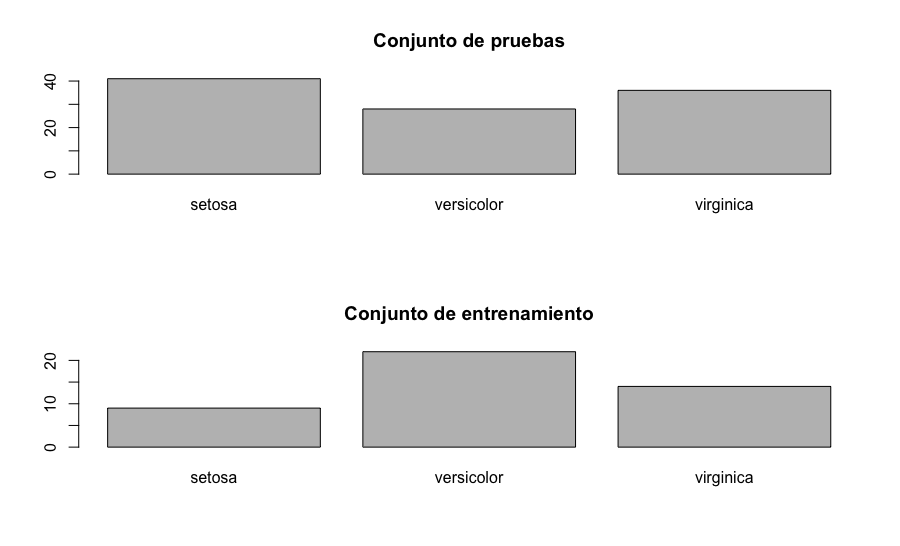
\includegraphics[width=1\textwidth]{fase8.png}
\caption{\label{fig:frog2}\textit{Número de observaciones por clase de iris. Del lado izquierdo se muestra el número de observaciones para el conjunto de pruebas y del lado derecho el número de observaciones el conjunto de entrenamiento.}}
\end{figure}

Se procede a ejecutar la validación del modelo, la aproximación que se muestra consiste en tomar el modelo que se ejecutó para la fase de entrenamiento (105 datos) y efectuar clasificaciones con la información nueva del conjunto de pruebas(45 datos). Este método permite conocer si el primer modelo para la fase de entrenamiento es suficiente o requiere ajustes. 

Para el caso de iris un modelo exitoso es aquel capaz de clasificar las tres clases de flores con un desempeño similar o mejor a la fase de entrenamiento. De acuerdo con la matriz de confusión se pueden identificar posibles fallos en los que el modelo no está siendo lo suficientemente sensible al reconocer una clase. La forma de medir el desempeño de este modelo se mide de acuerdo al número de clasificaciones erróneas respecto al total de la muestra; para el caso de la fase de entrenamiento un 2\% de error.

A continuación se muestra el resultado de la clasificación del modelo con la información en la fase de pruebas test\_set. Según la matriz de confusión, únicamente un valor es clasificado erróneamente y cerca del 98\% de los casos es identificado según la clase a la que realmente pertenece. El modelo muestra un desempeño adecuado y similar al set de entrenamiento por lo cual se tomará como un modelo apto para la clasificación automatizada.

\begin{lstlisting}
## Validacion del modelo LDA
## Se ejecutan las predicciones sobre
## el set de pruebas con el modelo original 
prediccion <- predict(modelo, newdata = test_set)

## Matriz de confusion
## Se muestran las clasificaciones correctas
## en la diagonal para el set de pruebas
table(prediccion$class, test_set$Species)
\end{lstlisting}

\begin{figure}[H]
\centering
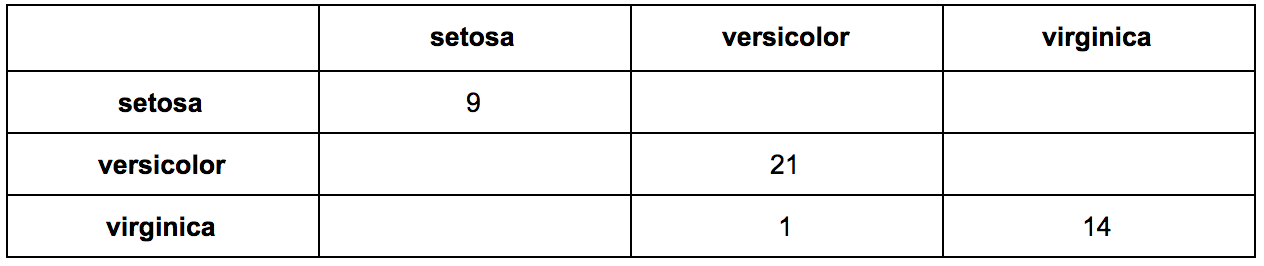
\includegraphics[width=1\textwidth]{fase9.png}
\caption{\label{fig:frog2}\textit{Matriz de confusión para el set de pruebas.}}
\end{figure}

Una vez corroborada la eficiencia del algoritmo de LDA para la fase de pruebas se puede considerar listo para clasificar más información sobre las tres especies de iris. Tomando en cuenta que el algoritmo de aprendizaje automático es útil para distinguir las tres especies de plantas en un caso de mayor escala. Para este sencillo ejemplo se analizaron 150 plantas, de las cuales 105 se utilizaron para entrenar el algoritmo y 45 para ponerlo a prueba. 

Probablemente en un ambiente mucho más cercano a la realidad los volúmenes de información sean cientos o miles de veces más grandes, sin embargo los mismos principios de muestreo, entrenamiento y prueba se mantienen. A continuación se muestra un caso con un volúmen de información más amplio y con un enfoque de análisis de mercados.

\subsection{Clasificación de clientes, caso de retail marketing}

Previamente se revisan los conceptos básicos del algoritmo de clasificación LDA. Se demuestra un caso práctico con cerca de 150 muestras para el famoso conjunto de datos del estadístico y biólogo Fisher (1936). Se explica un caso donde se clasifican 4 especies distintas de flores y se replica el experimento original que Fisher desarrolló en su momento. Aunque los principios que se atribuyen para el ejemplo práctico anterior, la complejidad del mundo actual exige análisis con información más elaborada y de modelización un poco más específica.

En esta sección se analiza un caso de información de transacciones internacionales en un esquema de proveeduría de mercancías a gran escala. Este sector de empresas es conocido como venta de retail y se caracteriza por manejar volúmenes a grandes escalas. Los datos pertenecen a una empresa de retail que opera en el Reino unido de forma Online de 2011 al 2011. La información a analizar consiste en cerca de 55,000 transacciones a nivel global para 38 países en 8 distintas variables, más de 4 millones de datos en un periodo de un año.

Uno de los objetivos más esenciales del marketing es segmentar los mercados. Una segmentación consiste en encontrar grupos de clientes actuales o potenciales que muestren características similares para enfocar alguna clase de producto específico según sus necesidades gustos y preferencias, entre otros como ubicación geográfica, cuestiones conductuales, etnográficas y culturales por ejemplo. Si bien, este ejercicio no pretende explicar ampliamente las diferentes características que existen en la segmentación de mercados ofrece una aplicación realista del método de segmentación LDA en función del comportamiento transaccional en cuanto a precio y cantidad de la transaccionalidad de la empresa.

El objetivo de este ejemplo es resolver un problema común en la actualidad. La información almacenada en equipos de cómputo no siempre son llevados a cabo con las mejores prácticas. Algunas empresas e instituciones de tamaño pequeño y mediano confían la información guardada en equipos locales, en bases de datos en hojas de cálculo. El manejo inadecuado de la información conlleva riesgos que pueden llegar a ser muy costosos. Un caso extremo es la empresa \textit{Newgg}, una empresa de retail que opera en California EE.UU. que en 2015 sufrió un ataque de hackers profesionales que demandaban un rescate en bitcoins, el servicio estuvo inactivo por 5 horas y algunas transacciones resultaron en pérdidas para la empresa. 

En este ejercicio, se simula la pérdida de información de transacciones a clientes que provienen de Polonia y Japón debido a un ataque de hackers que quieren destruir la empresa. Bajo el supuesto de que no se tienen los recursos para el rescate en bitcoins, los directivos deciden tomar el riesgo y utilizar algoritmos para recuperar parte de la información perdida.

El apartado permite brindar una opción para resolver la operación temporal de la empresa entrenando un algoritmo de inteligencia artificial capaz de clasificar los pedidos que provienen de Japón o Polonia. El ejemplo que se desarrolla en esta sección consiste en construir el algoritmo necesario para clasificar cuáles transacciones o ventas se originaron en cada uno de los países, así evitar costos innecesarios al enviar grandes cantidades de productos al país equivocado que podrían implicar pérdidas millonarias para la empresa. El algoritmo de clasificación LDA permite conocer el país de origen de las transacciones y establecer un plan de emergencia para satisfacer los pedidos de los clientes reduciendo el riesgo y por lo tanto grandes costos de hacer envíos incorrectos.

A continuación se carga la información en el ambiente para su posterior clasificación. De acuerdo con el código siguiente se transforma la información para evitar inconsistencias en los datos. Primero, se eliminan notas de crédito\footnote{ Una nota de crédito consiste en una devolución del producto posterior al momento de la compra. Generalmente, cuando una empresa otorga un producto se efectúa un plazo para que el cliente verifique que está en las condiciones y cantidades adecuadas. Por motivos contables, las cantidades se escriben negativas al momento de haber un pedido devuelto total o parcialmente. Esta situación es muy común en los negocios de retail ya que en volúmenes significativos los clientes solicitan crédito en tiempos de días de pago (30, 90 o 180 días para pagar).} al cargar el conjunto de datos. Segundo se selecciona una muestra para dos países Polonia y Japón para simplificar la explicación del modelo. Tercero, se grafica de forma exploratoria ambos países.

\begin{lstlisting}
## Marketing retail clients segmentation
## Fuente de informacion: https://archive.ics.uci.edu/ml/datasets/Online+Retail#

## Instalaccion de paquetes
install.packages("dplyr")
install.packages("MASS")
install.packages("caret")

library(dplyr)

## Se carga la informacion
df <- read.csv("Online Retail.csv", stringsAsFactors = F) %>% 
  filter(Quantity >0, UnitPrice > 0) ## Se eliminan devoluciones de producto (notas de compra)


## Se eligen dos paises
muestra <- df %>% filter(Country == "Poland" | Country == "Japan")
muestra$Country <- as.factor(muestra$Country)

## Grafica exploratoria
plot(muestra$Quantity, 
     muestra$UnitPrice, 
     col = as.factor(muestra$Country))
\end{lstlisting}

\begin{figure}[H]
\centering
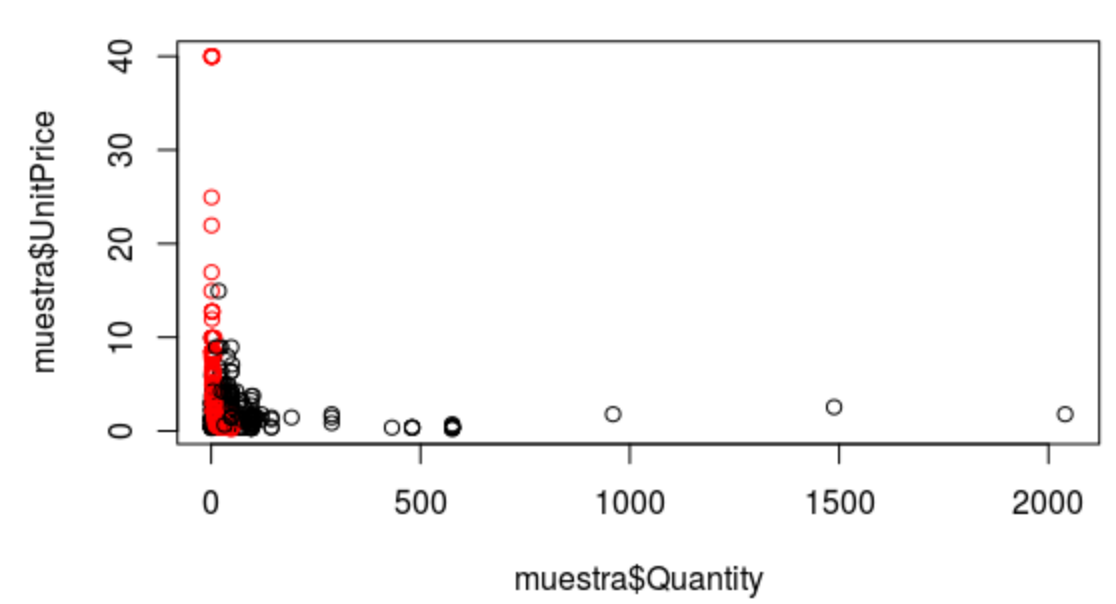
\includegraphics[width=1\textwidth]{marketing1.png}
\caption{\label{fig:frog2}\textit{Cantidad de producto vendido contra el precio del producto. Se muestran las compras provenientes de Polonia en color rojo y Japón en color negro.}}
\end{figure}

De acuerdo con la figura anterior se observa una concentración de la información cercano al origen para ambos ejes. La información cuya distribución no es uniforme es un caso típico de información real. Este tipo de dificultades resulta muy común en el análisis diario y es necesario llevar a cabo un pre procesamiento de la información para crear el algoritmo de LDA.

\subsection{Preprocesamiento de datos: escalamiento y normalización.}

El escalamiento de la información tiene como fin convertir los vectores de información que componen nuestro conjunto de información en una forma más susceptible de ser analizada. Para este caso específico, se observa una concentración poco favorable para el análisis en la figura X. Dentro de los métodos de escalamiento y normalización se encuentran las transformaciones logarítmicas, los escalamientos en función de máximos y mínimos, estandarización en función de la desviación estándar, entre otros. 

Para la mayoría de los casos en los que se aplica un algoritmo de inteligencia artificial este proceso es fundamental y en una gran cantidad de casos estrictamente necesario para obtener un modelo de clasificación aceptable. Sin embargo puede haber situaciones en la que no es necesario, en la sección anterior al clasificar el problema de Fisher 1936 no resultaba necesario el proceso de escalamiento por ejemplo.

De acuerdo una función logarítmica.

$$ y = log(x) $$

Donde x es un valor que se encuentra en el dominio de los reales positivos.

$$ x  \epsilon \mathbb{R} : x > 0 $$

Se cumplen los siguientes límites.

\begin{table}[H]
\centering
%%\caption{}
\label{my-label}
\begin{tabular}{lclcl}
\hline
Límite de la función              & Interpretación                                                   \\
\hline
$lim_{x\rightarrow 1} log(x) = 0$ & {\footnotesize Todo valor de x que tienda a 1 será 0 en el valor y.}  \\
\hline
$lim_{x\rightarrow 1} log(x) = 0$ & {\footnotesize Todo valor de x que tienda a infinito será infinito en valor y.} \\
\hline
$lim_{x\rightarrow 1} log(x) = 0$ & {\footnotesize Todo valor de x que tienda a 0 será menos infinito en el valor y.}\\
\hline
\end{tabular}
\end{table}

En la forma gráfica, se puede recrear la función logarítmica de la siguiente forma.

\begin{lstlisting}
## Grafica de la funcion logaritmica
## El dominio va de 0 a 5
plot(log, 0, 5, 
     main = "Funcion: y = log(x)", 
     xlab = "x", 
     ylab = "y")

## Especifica el punto donde x = 1
abline(v = 1, h = 0, lty = 3, col = "blue")
\end{lstlisting}

\begin{figure}[H]
\centering
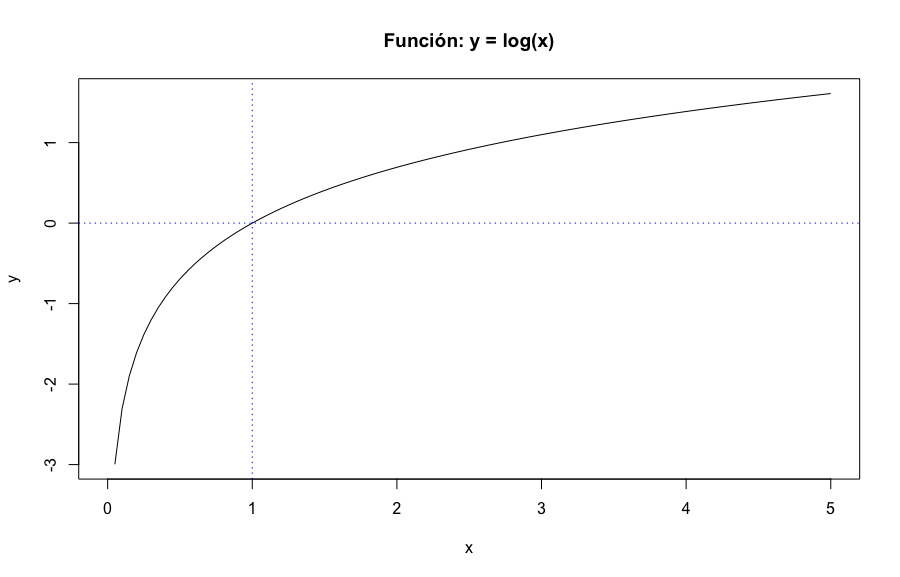
\includegraphics[width=1\textwidth]{log1.png}
%%\caption{\label{fig:frog2}\textit{Cantidad de producto vendido contra el precio del producto. Se muestran las compras provenientes de Polonia en color rojo y Japón en color negro.}}
\end{figure}

Al sustituir los valores x iguales a  1 se evita construir un nuevo vector y con valores iguales a 0 al aplicar la función logarítmica lo cual podría causar inconvenientes al efectuar el algoritmo de LDA e inconsistencias en la interpretabilidad del modelo. En este caso la función logarítmica se aplica a la cantidad de producto solicitado por el cliente y se evitan cantidades iguales a cero.

En este caso, se utiliza la transformación logarítmica para obtener una mejor distribución de la cantidad vendida y los precios de los productos. El objetivo es que la información sea accesible para análisis y entrenamiento del algoritmo de LDA. El proceso consiste en aplicar la función logarítmica base 10 o logaritmo natural al vector de precios y al vector de cantidades como se describe a continuación.

\begin{lstlisting}
## Se reescala la informacion en logaritmos
muestra$Quantity[muestra$Quantity == 1] <- 2

## Construccion de los vectores de logaritmos
muestra$log_Quantity     <- log(muestra$Quantity)
muestra$log_UnitPrice    <- log(muestra$UnitPrice)

## Colores por pais
plot(muestra$log_Quantity, muestra$log_UnitPrice, col = muestra$Country)
\end{lstlisting}

\begin{figure}[H]
\centering
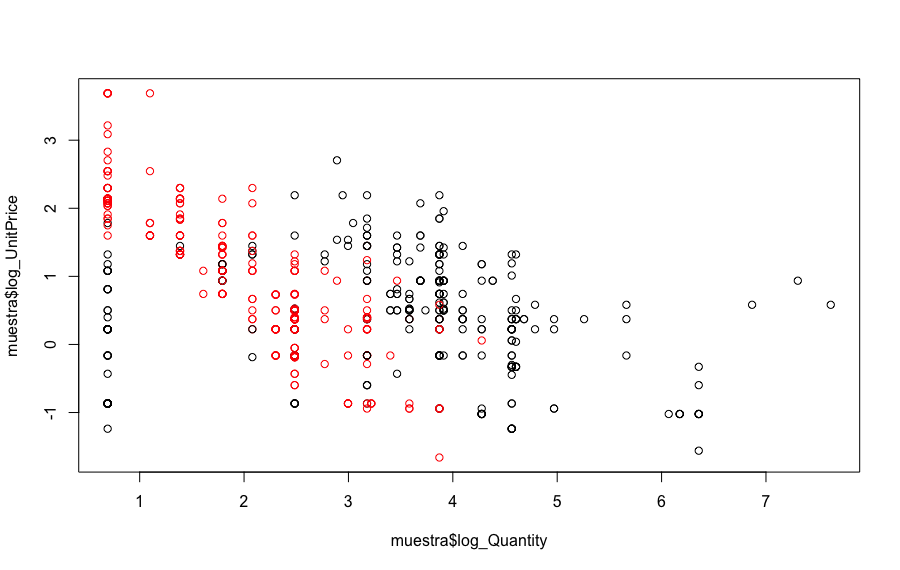
\includegraphics[width=1\textwidth]{marketing2.png}
\caption{\label{fig:frog2}\textit{Logaritmos de producto vendido contra el precio del producto. Se muestran las compras provenientes de Polonia en color rojo y Japón en color negro.}}
\end{figure}

Como se observa en la figura X, la información bajo la transformación logarítmica es razonablemente más entendible que el caso de la figura X-1. De acuerdo con la gráfica anterior se intuye que Japón es un cliente cuya demanda de productos es más alta que Polonia al estar más alejado del origen en términos de cantidad y de precio.

Al realizar la transformación logarítmica el algoritmo de LDS será más preciso al efectuar la clasificación supervisada. 

\subsection{Fase de entrenamiento}

El set de entrenamiento o \textit{training set} consiste en una sección de la información que será utilizada para entrenar el modelo de segmentación. Como se menciona en algoritmo anterior una forma simple es utilizar una selección aleatoria de una porción determinada de la información, de esta forma se puede utilizar una parte suficiente para entrenar el modelo.

\begin{lstlisting}
## Fase de entrenamiento
## Seleccion del 70% de la informacion

porcentaje <- 70/100

num_muestras <- porcentaje * nrow(muestra)

set.seed(4)
train_ind <- sample(seq_len(nrow(muestra)), size = num_muestras)

## Seleccionamos las muestras que pertenecen
## al set de entrenamiento
train_set <- muestra[train_ind, ]

## Seleccionamos el resto de muestras
## que pertenecen al set de pruebas
test_set <- muestra[-train_ind, ]
\end{lstlisting}

Otra ventaja de este muestreo simple es que permite entrenar el modelo de LDA en una porción de la información y validar el modelo en el resto de los datos (usualmente de menor tamaño). En la figura X se explica cómo se divide la información para el caso de las especies iris. Para el caso del retail shop, hay 445 datos para el set de entrenamiento (70\% de la información) y 196 casos para validar el modelo.

A continuación se efectúa el entrenamiento y las predicciones del modelo de LDA. El código efectúa las predicciones para el set de entrenamiento y de forma gráfica se verifica que la clasificación represente una clasificación adecuada. En la figura siguiente se muestra del lado izquierdo los resultados de clasificación del algoritmo propuesto. Por otro lado, del lado derecho se observan las categorías originales a las que pertenece cada uno de los puntos. 

\begin{lstlisting}
## Ejecucion del algoritmo de LDA

library(MASS)
library(caret)
par(mfrow=c(1,2)) ## Se especifica que se quieren dos graficas en un mismo renglon


modelo <- lda(data =train_set, Country ~.)
prediccion <- predict(modelo, type = "Class")
plot(prediccion$x, col =prediccion$class, main = "Prediccion")
plot(prediccion$x, col =train_set$Country, main = "Original")
\end{lstlisting}

\begin{figure}[H]
\centering
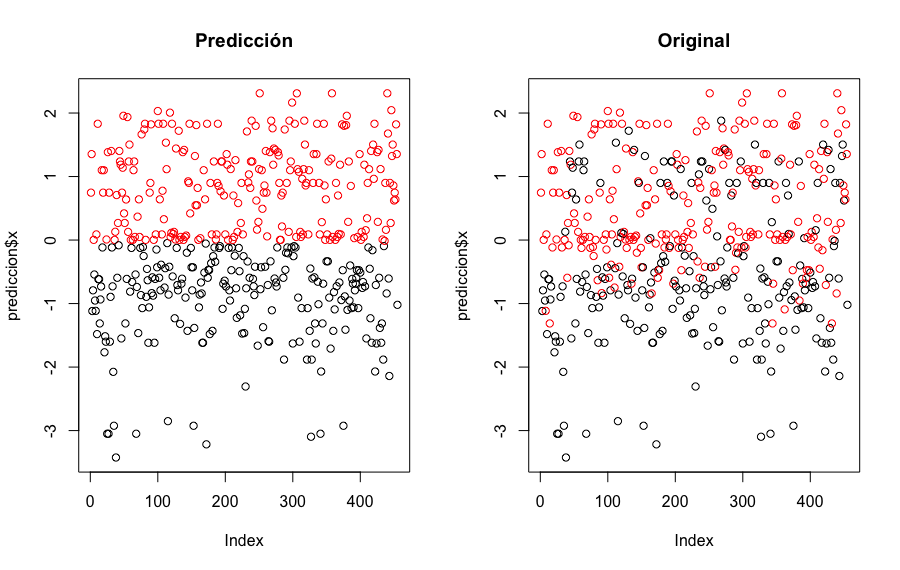
\includegraphics[width=1\textwidth]{marketing3.png}
\caption{\label{fig:frog2}\textit{Clasificación de clientes según modelo clasificatorio LDA. Del lado izquierdo se muestra la clasificación efectuada por el algoritmo y del lado derecho se muestran los casos reales.}}
\end{figure}

El método de validación gráfico anterior es válido para explorar la información, encontrar tendencias u observar errores evidentes. Sin embargo, aunque un modelo clasificatorio luzca aparentemente adecuado es necesario realizar una prueba del desempeño del algoritmo conocido como validación. La validación se realiza en la sección restante de información que se seleccionó aleatoriamente al crear el set de entrenamiento y el set de pruebas. 

En el set de pruebas se utiliza el modelo previamente entrenado para intentar predecir las categorías a las que pertenece cada uno de los clientes. En este caso el modelo entrenado tratará de predecir si el pedido pertenece a Japón o a Polonia de acuerdo a las variables previamente definidas como volumen de mercancías y precio. 

Aunque un modelo resulte aceptable dentro del set de entrenamiento, la validación empírica es siempre deseable. Para ello, se utiliza el set de pruebas y se mide el desempeño del modelo en una fracción de la información que simula un caso real de información nueva. A continuación se mide el desempeño del algoritmo en función de cuántos casos son correctamente clasificados.

\begin{lstlisting}
## Matriz de confusion

prediccion <- predict(modelo, newdata = test_set)

matriz_confusion <-table(prediccion$class, test_set$Country)

confusionMatrix(matriz_confusion)
\end{lstlisting}

\begin{figure}[H]
\centering
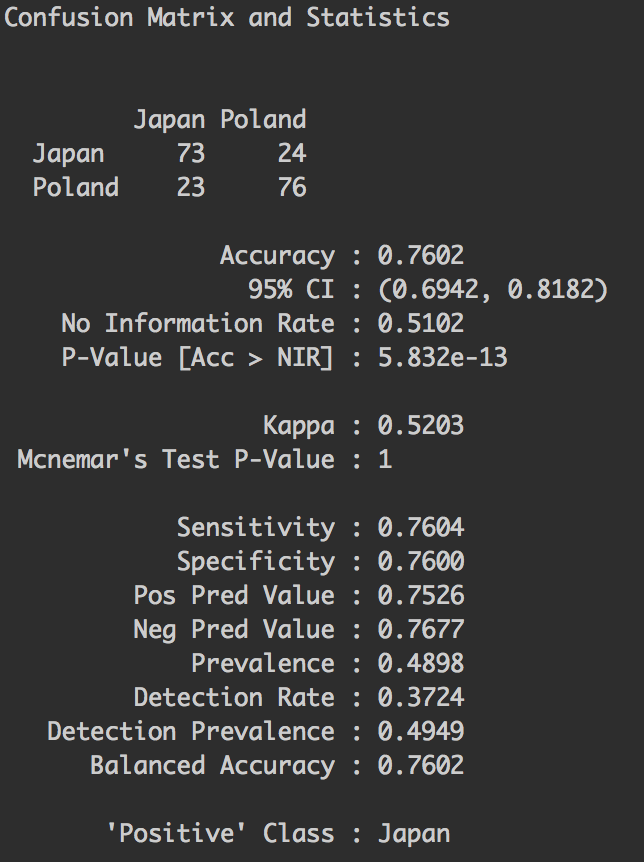
\includegraphics[width=0.5\textwidth]{marketing4.png}
\caption{\label{fig:frog2}\textit{Matriz de confusión}}
\end{figure}


El estadístico utilizado es conocido como matriz de confusión. Un ejemplo y desarrollo de sus usos se encuentran en la sección anterior para el caso de clasificación de especies biológicas. En resumen, la matriz de confusión indica el número de predicciones que fueron acertadas así como el número de aquellas que fueron clasificadas erróneamente. Para este caso se utiliza el valor de precisión del modelo, el estadístico accuracy va de 0 a 100\% siendo 100\% clasificación sin errores y 0\% clasificación totalmente errada. 

El ejercicio de clasificación anterior muestra un 76\% de los casos correctamente clasificados. Valores de sensibilidad del 76\% y especificidad de la misma magnitud. De acuerdo con AUTORES LOCOS el desempeño de un algoritmo de clasificación resulta bueno cuando estos valores son cercanos al 80\%.

En este ejemplo, se logra clasificar adecuadamente cerca de 200 transacciones. De acuerdo al planteamiento inicial de este apartado se podrá ofrecer una perspectiva de inteligencia artificial para poder identificar algunas de las órdenes de compra que provengan de los países analizados. 

El algoritmo de LDA permite reducir el riesgo y por lo tanto costos de enviar cargamentos de mercancías al otro lado del mundo de forma incorrecta. La clasificación que se efectúa con una sección de la información como fase de entrenamiento es suficiente para poder desarrollar un modelo que tiene la capacidad de segmentar si un pedido se originó en Japón o Polonia.

\chapter{Algoritmos predictivos}

En esta sección se desarrollan algunas de las populares técnicas de predicción en el campo de la inteligencia artificial de tipo aprendizaje automático o machine learning. En el apartado anterior se desarrollan algoritmos de clasificación lineal con la finalidad de categorizar información dadas ciertas características (principalmente, pero no exclusivamente) cuantitativas. En la primera sección se desarrollan los principios básicos para identificar los tres casos en los que se utilizan las técnicas de inteligencia artificial que componen este apartado.

De acuerdo con el capítulo uno se pueden identificar tres clases esenciales de algoritmos de machine learning, segmentación, identificación y predicción. Los algoritmos de predicción resultan ser especialmente atractivos debido a que pueden ser utilizados en un sin fin de situaciones. Entre algunas de estas utilidades se encuentra conocer los precios de ciertas emisoras de bolsa con un bajo grado de incertidumbre, conocer los niveles esperados de audiencia en una plataforma de Marketing digital, modelar expectativas y definir rango de “normalidad” para detectar anomalías en un sistema. Algunos otros usos de los métodos de predicción: conocer el comportamiento de clientes potenciales en un esquema de interacciones en línea o inclusive deducir comportamiento de una muestra poblacional para tomar decisiones y efectuar cierta medida.

Una gran parte de los escritos consideran las técnicas de predicción un tema intermedio dentro de las ramas de ciencias computacionales y la ciencia económica. Si bien, desarrollar un sistema que realice las funciones de predicción dado un algoritmo de machine learning no es una tarea sencilla\footnote{ara todo aquel entusiasta de los retos intelectuales, el director del laboratorio de inteligencia artificial de Stanford Andrew Ng ofrece la clase de maestría de de Machine Learning, el curso se encuentra disponible de forma gratuita en la plataforma de Coursera. Resulta un buen punto de partida para conocer las dificultades que conlleva construir los algoritmos de inteligencia artificial y aprender más allá del uso práctico que se ofrece en este texto.} a diferencia de otros textos especializados, el objetivo de este libro no es profundizar en los principios estadístico-matemáticos y computacionales que fundamentan esta clase de inteligencia artificial. 

Afortunadamente, para un nivel introductorio conocer a detalle los métodos conlleva una gran dedicación al ser temas ajenos a cualquier ciencia social. Sin embargo, aprender a utilizar las herramientas y reforzar la teoría más adelante permite comenzar a desarrollar habilidades en el tema. Este sistema de exposición, popular entre los manuales técnicos y otros textos, ayudan a brindar un contexto práctico.  

Por otro lado, este texto y la subsecuente sección pretende mostrar el uso de las herramientas ya desarrolladas con un enfoque funcional para el uso cotidiano en las ciencias sociales.

\section{Contexto histórico}

Desarrollar al máximo el campo de la predicción ha sido una de los máximos objetivos del ser humano desde tiempos ancestrales. Los primeros seres humanos que poblaron la tierra crearon intrincados sistemas astrales con el fin de predecir las mejores tiempos de siembra, cosecha y recolecta durante los principios de la dinámica sedentaria. En épocas tempranas del desarrollo técnico, se crearon los primeros sistemas de medición-determinación del tiempo\footnote{Por ejemplo, el reloj astronómico de Praga fue construído a principios del siglo XV con el fin de predecir equinoccios, días festivos, épocas ideales de siembra y cosecha.} con el fin de obtener información con antelación sobre eventos por suceder. 

El transcurso del tiempo permitió el desarrollo de las fuerzas productivas y con el crecimiento de la riqueza a nivel mundial los mercados de transacción y producción de mercancías florecieron, el hombre deseaba conocer de antemano los precios de los productos para obtener un beneficio al realizar un ciclo de producción e intercambio. Resulta evidente que aquellos poseedores de información precisa sobre los precios tenían una comercial ventaja significativa en el comercio sobre aquellos que formulaban predicciones incorrectas. Hoy en día los usos de un sistema (o modelo) predictivo es valioso para prácticamente todas las industrias, sin embargo la sofisticación de la técnica estadístico-matemática y computacional pone el arte de predecir en contexto radicalmente distinto.

Bajo el contexto económico actual la información juega un papel crucial más acelerado que en épocas anteriores. Tener la capacidad de predecir el comportamiento de cierto fenómeno incurre en ganancias o en terribles pérdidas en caso de manejarse de forma incorrecta. Para el caso de las ciencias médicas, identificar cierto tipo de patología con un modelo de predicción erróneo puede significar someter a un paciente a un tratamiento que no necesita o en cambio, no detectar la patología y no ofrecer ningún tipo de tratamiento a un paciente enfermo. La necesidad de buenas predicciones nacen de distintas perspectivas, sin embargo las implicaciones de efectuar un pronóstico equivocado son relevantes para la mayoría de los casos.

En esta sección, se revisan distintos modelos predictivos simples que siguen los principios de inteligencia artificial previamente descritos. En general, cualquier tipo de algoritmo predictivo de inteligencia artificial actual se considera un tema avanzado de modelización. Usualmente siquiera en cursos de posgrado de Ciencias Sociales son contemplados como parte esencial y un adecuado conocimiento sobre los fundamentos del mismo no siempre es adquirido. Si bien, las herramientas tecnológicas que nos permiten ejecutar modelos avanzados, conocer los principios es siempre recomendado.

Este texto pretende ofrecer una visión básica e introductoria a predicción por medio de algoritmos de inteligencia artificial, una perspectiva más amplia puede encontrarse en textos especializados e inclusive títulos específicos del algoritmo que se desea emplear. En esta sección se utilizarán dos versiones de algoritmo predictivo redes neuronales artificiales y un modelo econométrico tradicional de vectores de autorregresivos con órdenes de integración (ARIMA). 

Los métodos previamente mencionados resultan ser herramientas útiles para predecir. Especialmente, las redes neuronales artificiales son conocidas por mostrar un buen desempeño de predicción para casos donde la información se presenta de forma continua (series de tiempo o información estructurada). Dominar ambas perspectivas, conocer modelos econométricos tradicionales como ARIMA y al mismo tiempo conocer sobre redes neuronales artificiales, permite conocer un espectro básico pero suficiente para comenzar a efectuar algunas aplicaciones simples de inteligencia artificial.

\section{Redes neuronales artificiales}

Las redes neuronales artificiales nacen de la abstracción sobre las neuronas que existen en los sistemas biológicos dada su funcionalidad de aprendizaje. Para el caso de redes neuronales artificiales, se asemejan a simular el funcionamiento de un conjunto de neuronas biológicas. Algunas aplicaciones de esta técnica de modelización pueden observarse en sistemas financieros, detección de anomalías en seguridad de sistemas e incluso vehículos de conducción asistida o conducción autónoma (Dasgupta et al, 2011; Shen et al 2008; Textor, 2012). Las ventajas principales de esta técnica residen en efectuar relaciones complejas, ya sean lineales o no lineales bajo la estimación de parámetros de aprendizaje (Hastie, 2009). Esto quiere decir, el modelo busca relaciones en la información y trata de aprender de los errores de forma iterativa.

Una neurona biológica, se compone de diferentes partes. En la figura siguiente se muestran las secciones de la neurona. El funcionamiento radica en la transmisión de información de la dendrita al núcleo. A su vez, esta información viaja al axón. El objetivo del núcleo es procesar esta información y se transfiere a la prolongación del soma neuronal (Paniagua et al, 2002).

\begin{figure}[H]
\centering
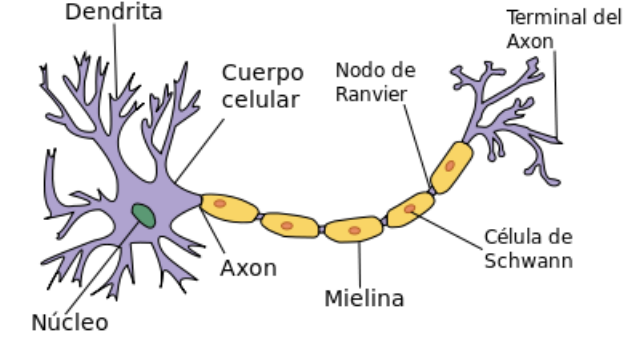
\includegraphics[width=1\textwidth]{neurona0.png}
\caption{\label{fig:frog2}\textit{Esquema de neurona biológica.}}
\end{figure}

Para el caso de una red neuronal artificial, es un conjunto de diversas neuronas que siguen este principio de transmisión de información. En un modelo de redes neuronales artificiales se determinan distintas capas (conjunto de neuronas) a las cuales se le transmite la información. Gráficamente, la representación de una red neuronal artificial se especifica de la siguiente manera.

\begin{figure}[H]
\centering
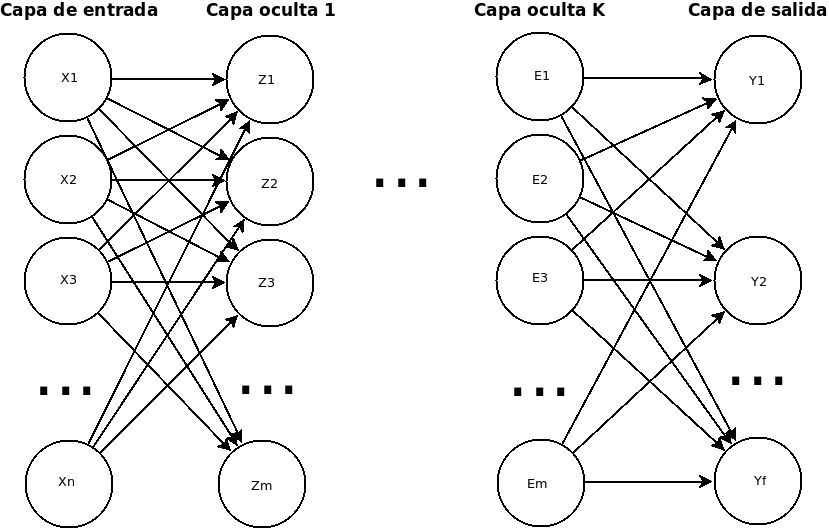
\includegraphics[width=1\textwidth]{neuralnetwork.png}
\caption{\label{fig:frog2}\textit{Estructura de Red Neuronal multicapa para f variables objetivo (Y). Fuente Olguín (2017).}}
\end{figure}

A continuación en este apartado se utilizará una red neuronal artificial para predecir el precio de las acciones de una emisora con un periodo diario. Se comparará la precisión del modelo de redes neuronales respecto a un método tradicional de forecasting popularmente conocido como ARIMA (Autoregressive integrated moving average) de forma estadística y gráfica. El desempeño de los modelos se medirán por el nivel de error que cada uno provee, menor error de predicción corresponderá al modelo más preciso. 

\subsection{Predicción de precio de acciones con redes neuronales artificiales}

Así como en las secciones anteriores del texto, el primer paso que se desarrolla es la obtención de la información a analizar. Para ello se utiliza el paquete quantmod (Ryan et al, 2017) que nos permite extraer información sobre las cotizaciones diarias \footnote{Adicionalmente, este paquete contiene un API para obtener información del famoso repositorio de datos Federal Reserve Economic Data (FRED). } de las emisoras más populares. Para este caso, se obtienen los precios de cierre y se grafica la figura de velas o candlestick chart.

\begin{lstlisting}
## Descargando la informacion
library(quantmod)
getSymbols("GOOG",src="google")
## Grafica quantmod
barChart(GOOG)
\end{lstlisting}

\begin{figure}[H]
\centering
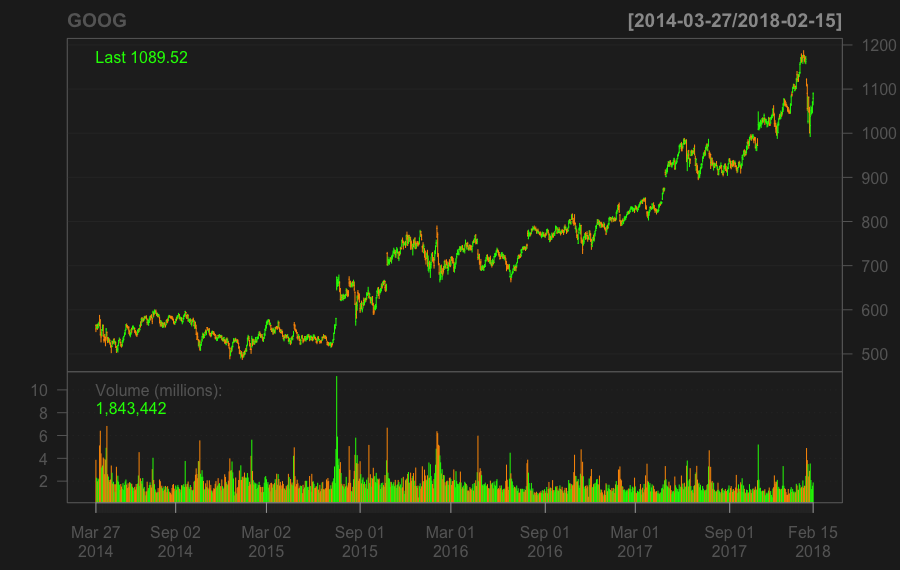
\includegraphics[width=1\textwidth]{google1.png}
\caption{\label{fig:frog2}\textit{Precio diario de la Alphabet Inc (Google) 2014-2018.}}
\end{figure}

Una vez visualizada la información, se puede seleccionar la variable objetivo a entrenar el modelo de redes neuronales. Siguiendo los principios de la fase de pruebas explicados en el capítulo dos, el set de entrenamiento o training set consiste en una sección de la información (en este caso una porción de la serie de tiempo) que será utilizada para entrenar o ajustar el modelo predictivo de series de tiempo. Para el caso de series de tiempo, es importante elegir de forma ordenada la información\footnote{A diferencia de los algoritmos de clasificación ejemplificados previamente que se caracterizan por su atemporalidad, un algoritmo o modelo de series de tiempo requiere una segmentación ordenada y no una selección aleatoria de la información.}, la segmentación ordenada resulta ser el método más simple para este caso. 

En el código que se muestra a continuación se observa el proceso de transformación de la información necesaria para entrenar el modelo. Posteriormente, se toman observaciones para entrenar el modelo que corresponden a la primera sección de la información. Además, se eligen 11 observaciones para probar el desempeño del modelo.

\begin{lstlisting}
df[(nrow(GOOG)-num_test_days):nrow(GOOG), ]
df.test.values <- df.test$GOOG.Close[1:num_test_days] 
df.test$d## Extrayendo la informacion a un data frame
df <- as.data.frame(GOOG)

## Se selecciona el numero de dias a predecir
num_test_days <- 10

## Se divide el set de entrenamiento
## Se eligen 191 observaciones para entrenar el modelo
df.train <- df[(nrow(GOOG)-200):(nrow(GOOG)-num_test_days), ]
df.train$days <- as.Date(row.names(df.train))

## Se selecciona la seccion que corresponde al set de pruebas
## Se eligen 11 observaciones (las mas recientes) para probar
## el desempeno del modelo
df.test <-ays <- as.Date(row.names(df.test))

## Se grafican los precios de cierre
plot(df.train$days, 
     df.train$GOOG.Close, 
     type = "l", 
     main = "Precio diario de la emisora Alphabet Inc (Google)")
\end{lstlisting}

\begin{figure}[H]
\centering
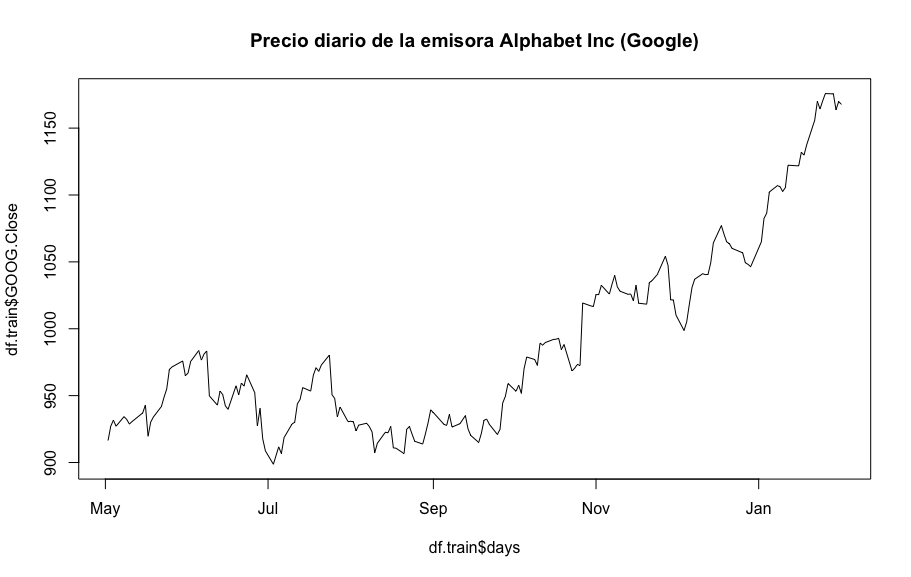
\includegraphics[width=1\textwidth]{Google2.png}
\caption{\label{fig:frog2}\textit{Precio diario al cierre de la Alphabet Inc (Google) correspondiente al set de entrenamiento.}}
\end{figure}

A continuación se ejecuta el modelo de redes neuronales artificiales. En principio, se definen el número de capas ocultas e iteraciones como dos capas ocultas y cinco mil iteraciones. Se selecciona la opción de escalamiento automático (scale.inputs) debido a que cualquier modelo de redes neuronales requiere rescalamiento de la información para ajustar adecuadamente el modelo. \footnote{ En la segunda sección del texto se profundiza en un caso de escalamiento manual con logaritmos. Para este caso se utiliza la transformación Box-Cox (Li, 2005).} En caso de seleccionar la opción scale.inputs = FALSE el desempeño del modelo es muy bajo para este caso.

\begin{lstlisting}
library(forecast)

## Ajuste del modelo
par(mfrow=c(2,1))
fit.nn <- nnetar(df.train$GOOG.Close, size = 2, repeats = 5000, scale.inputs = TRUE) 

## Ajuste del modelo de redes neuronales
fcast.nn <- forecast(fit.nn, h = num_test_days)

## Grafica de las predicciones
plot(fcast.nn)
lines(fitted(fcast.nn), 
      col = "red") ## se grafica el ajuste de entrenamiento en rojo

## Tabla resumen de desempeno del modelo
accuracy.nn <-as.data.frame(accuracy(fcast.nn$mean, x = df.test.values ))

## Ajuste del modelo arima
fit.arima <-auto.arima(df.train$GOOG.Close)
fcast.arima <- forecast(fit.arima, h = num_test_days)
plot(fcast.arima)
lines(fitted(fit.arima), col = "green")

accuracy.arima <- as.data.frame(accuracy(fcast.arima$mean, x = df.test.values))

accuracy.table<-rbind(accuracy.nn, accuracy.arima)
row.names(accuracy.table) <- c("Red Neuronal", "ARIMA")
accuracy.table
\end{lstlisting}

\begin{figure}[H]
\centering
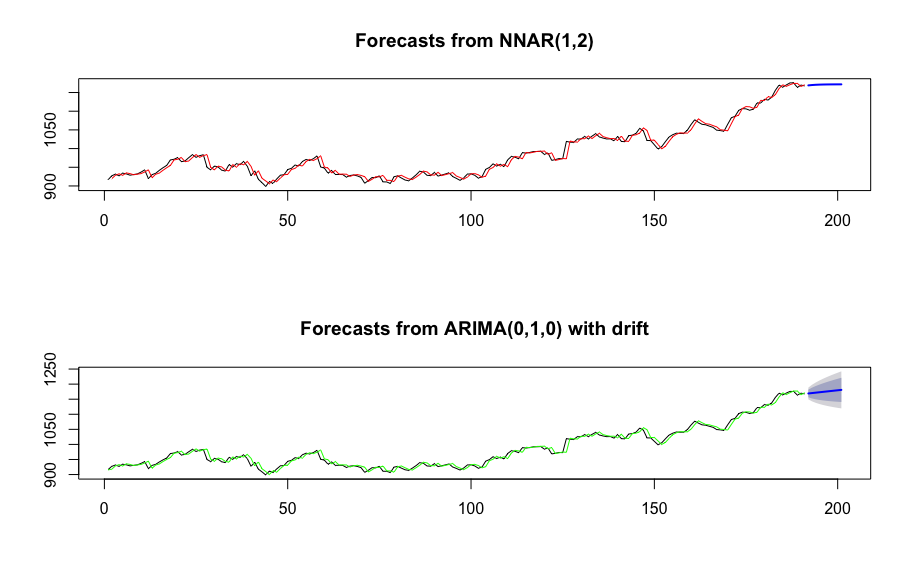
\includegraphics[width=1\textwidth]{Google3.png}
\caption{\label{fig:frog2}\textit{Modelo de redes neuronales artificiales (arriba) y modelo ARIMA (abajo) para el precio diario al cierre de la Alphabet Inc (Google) correspondiente al set de entrenamiento (negro). Se observa el ajuste del modelo en rojo para ambos casos y en azul los valores de la predicción.
}}
\end{figure}

Para llevar a cabo una comparación precisa del desempeño de los modelos se muestran las tablas resumen de error de cada modelo respecto a la sección de la información de pruebas. Una interpretación rápida muestra que el MAPE (Error Porcentual Absoluto Medio) es significativamente más bajo en el modelo de redes neuronales respecto al modelo ARIMA.

\begin{figure}[H]
\centering
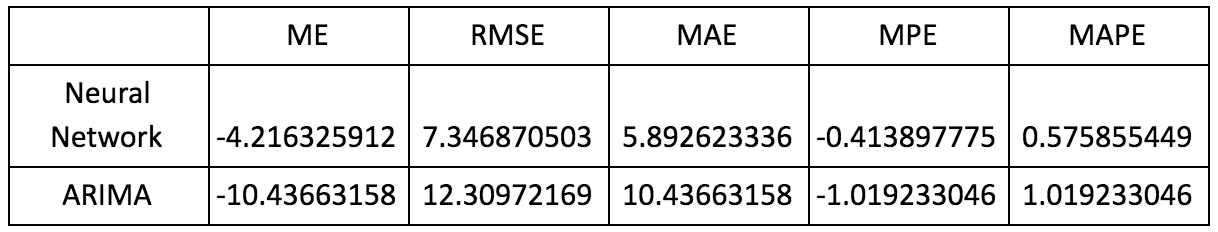
\includegraphics[width=1\textwidth]{google_performance.png}
%%\caption{\label{fig:frog2}\textit{}}
\end{figure}

Generalmente, un modelo cuyo error más bajo es un mejor modelo para predecir. Al medir el desempeño del modelo respecto a la sección de información de pruebas permite simular un escenario realista donde el modelo se confronta con la realidad. En la tabla anterior, se muestran errores más bajos para la red neuronal en todas las métricas de desempeño presentadas.


\end{document}



